\section*{Residuos y raíces}
\noindent Se guarda $y^2\bmod p$ en un arreglo; la otra raíz es $p-y$.
\begin{center}
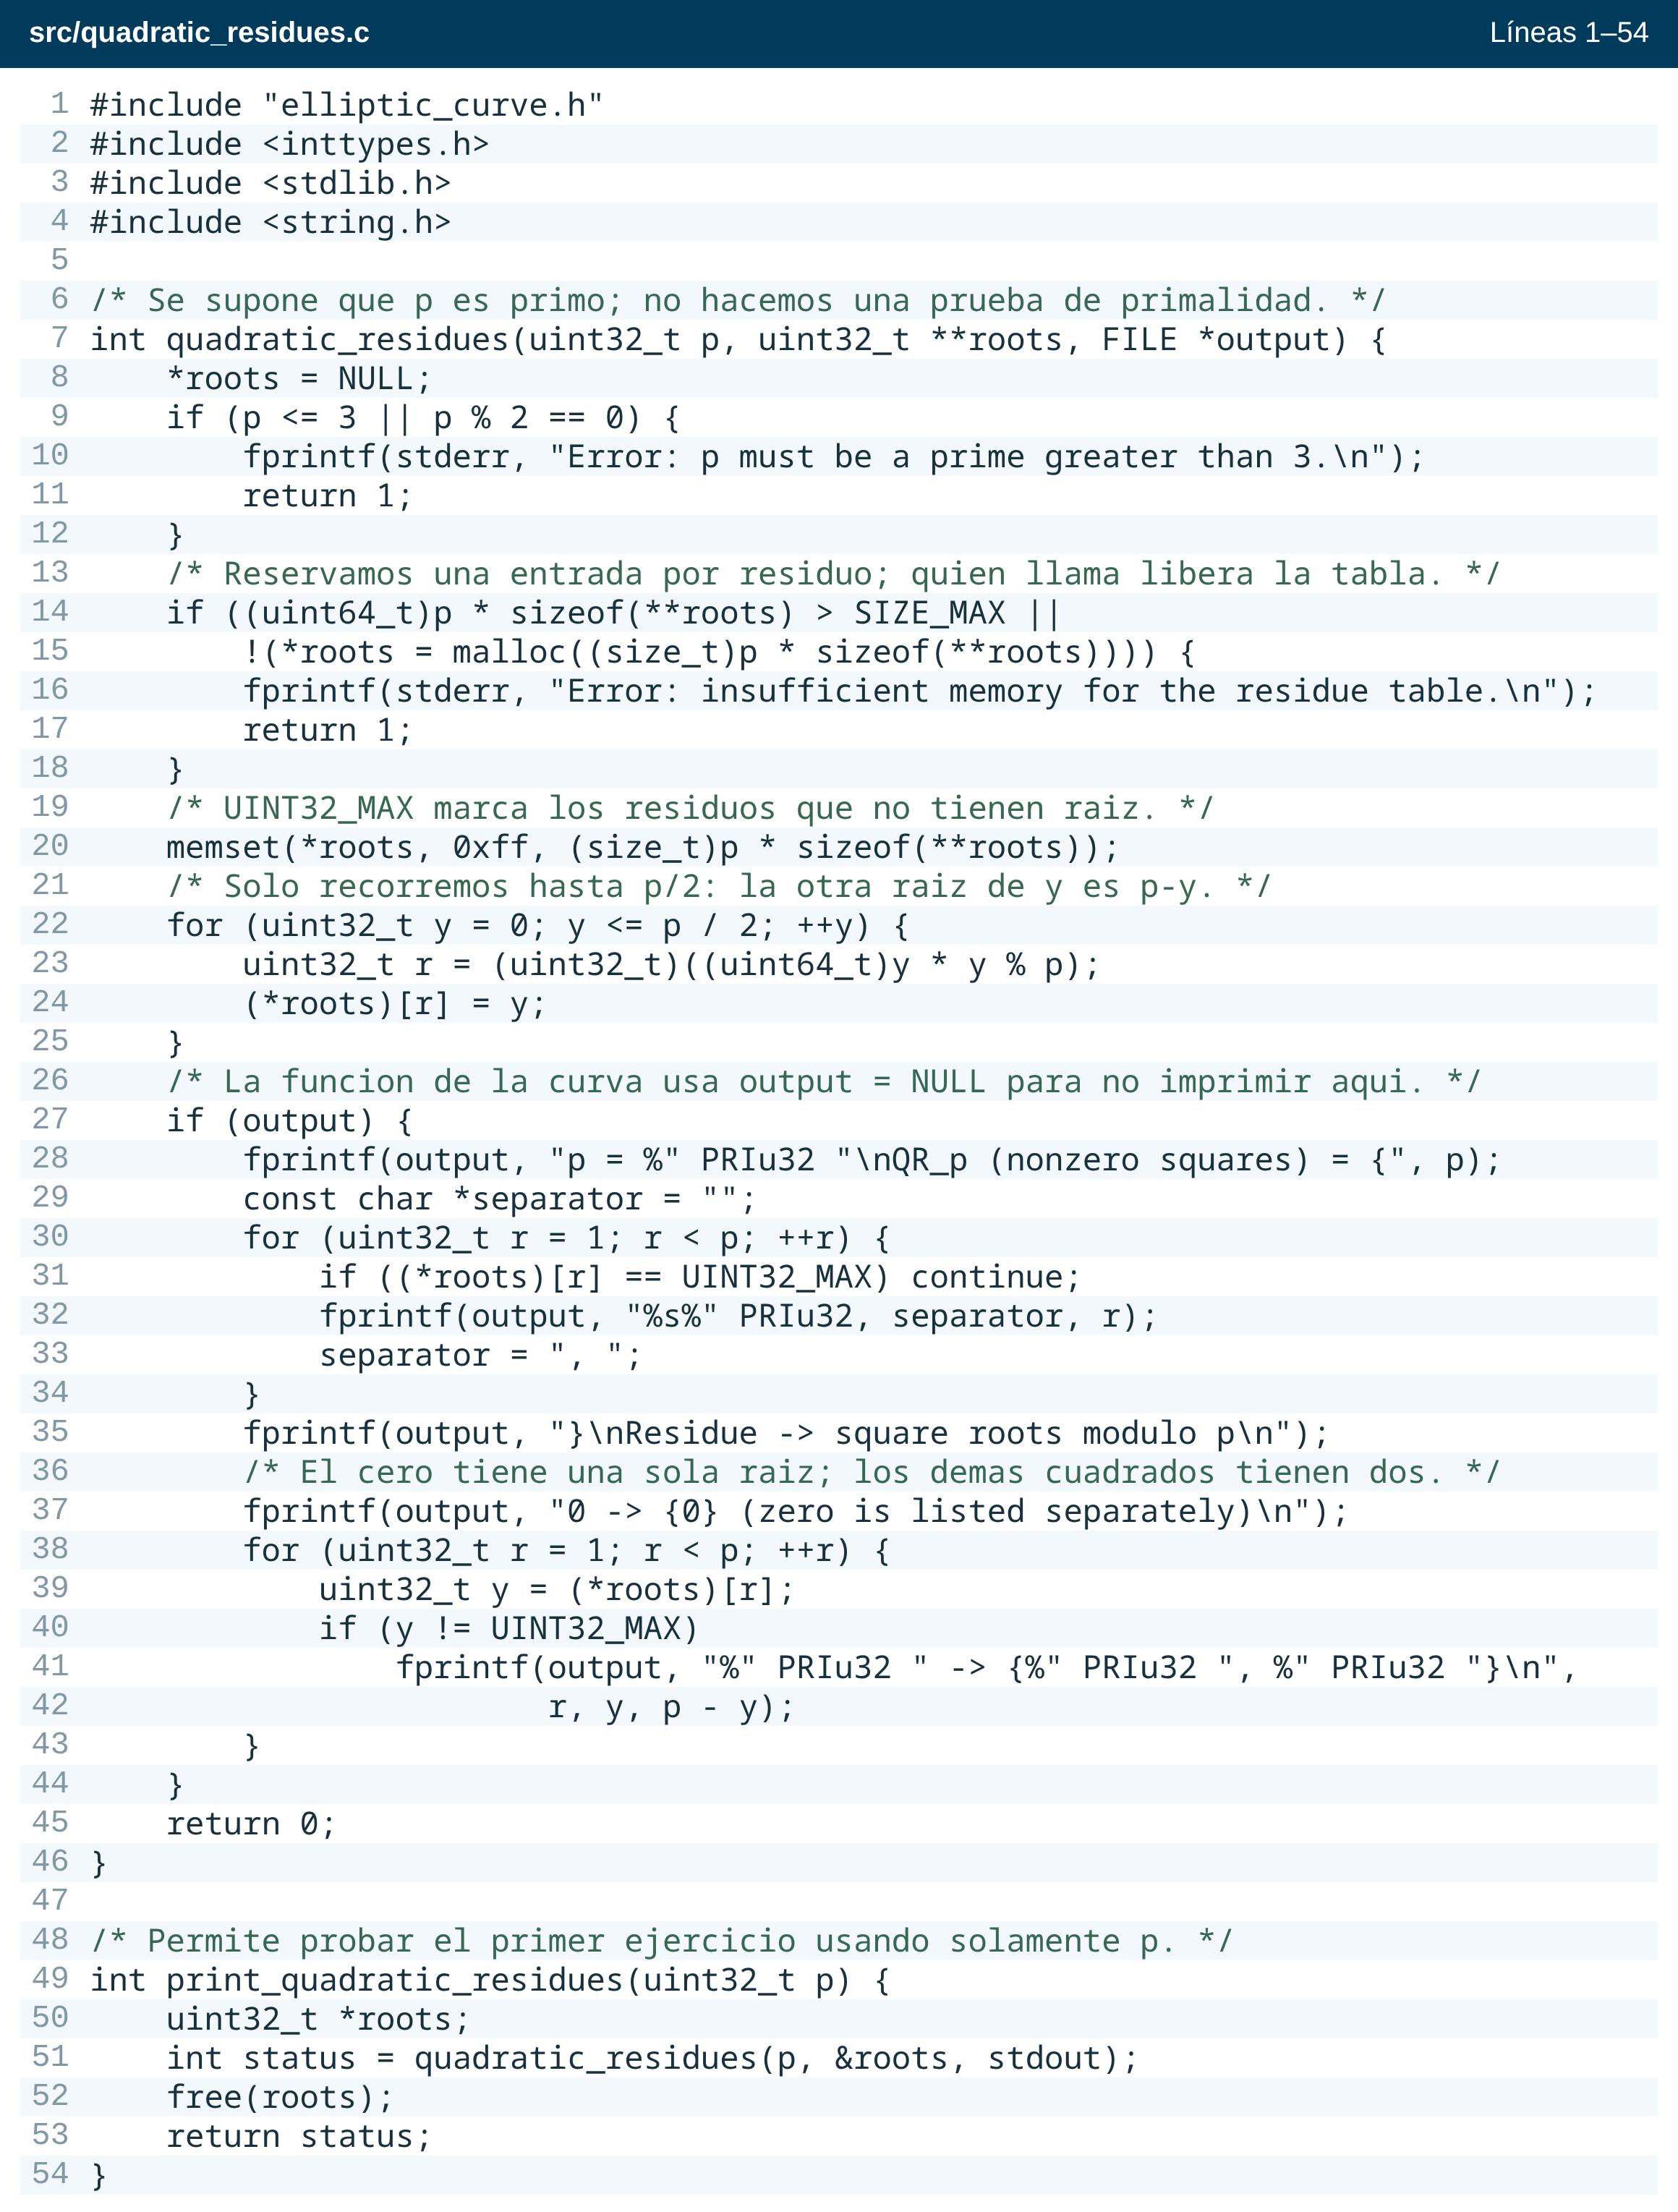
\includegraphics[width=\linewidth,height=0.85\textheight,keepaspectratio]{assets/capturas/final-residuos.png}
\end{center}
\clearpage
\section*{Evaluación y salida de puntos}
\noindent Para cada $x$, se busca la raíz de $x^3+ax+b\bmod p$ en el arreglo.
\begin{center}
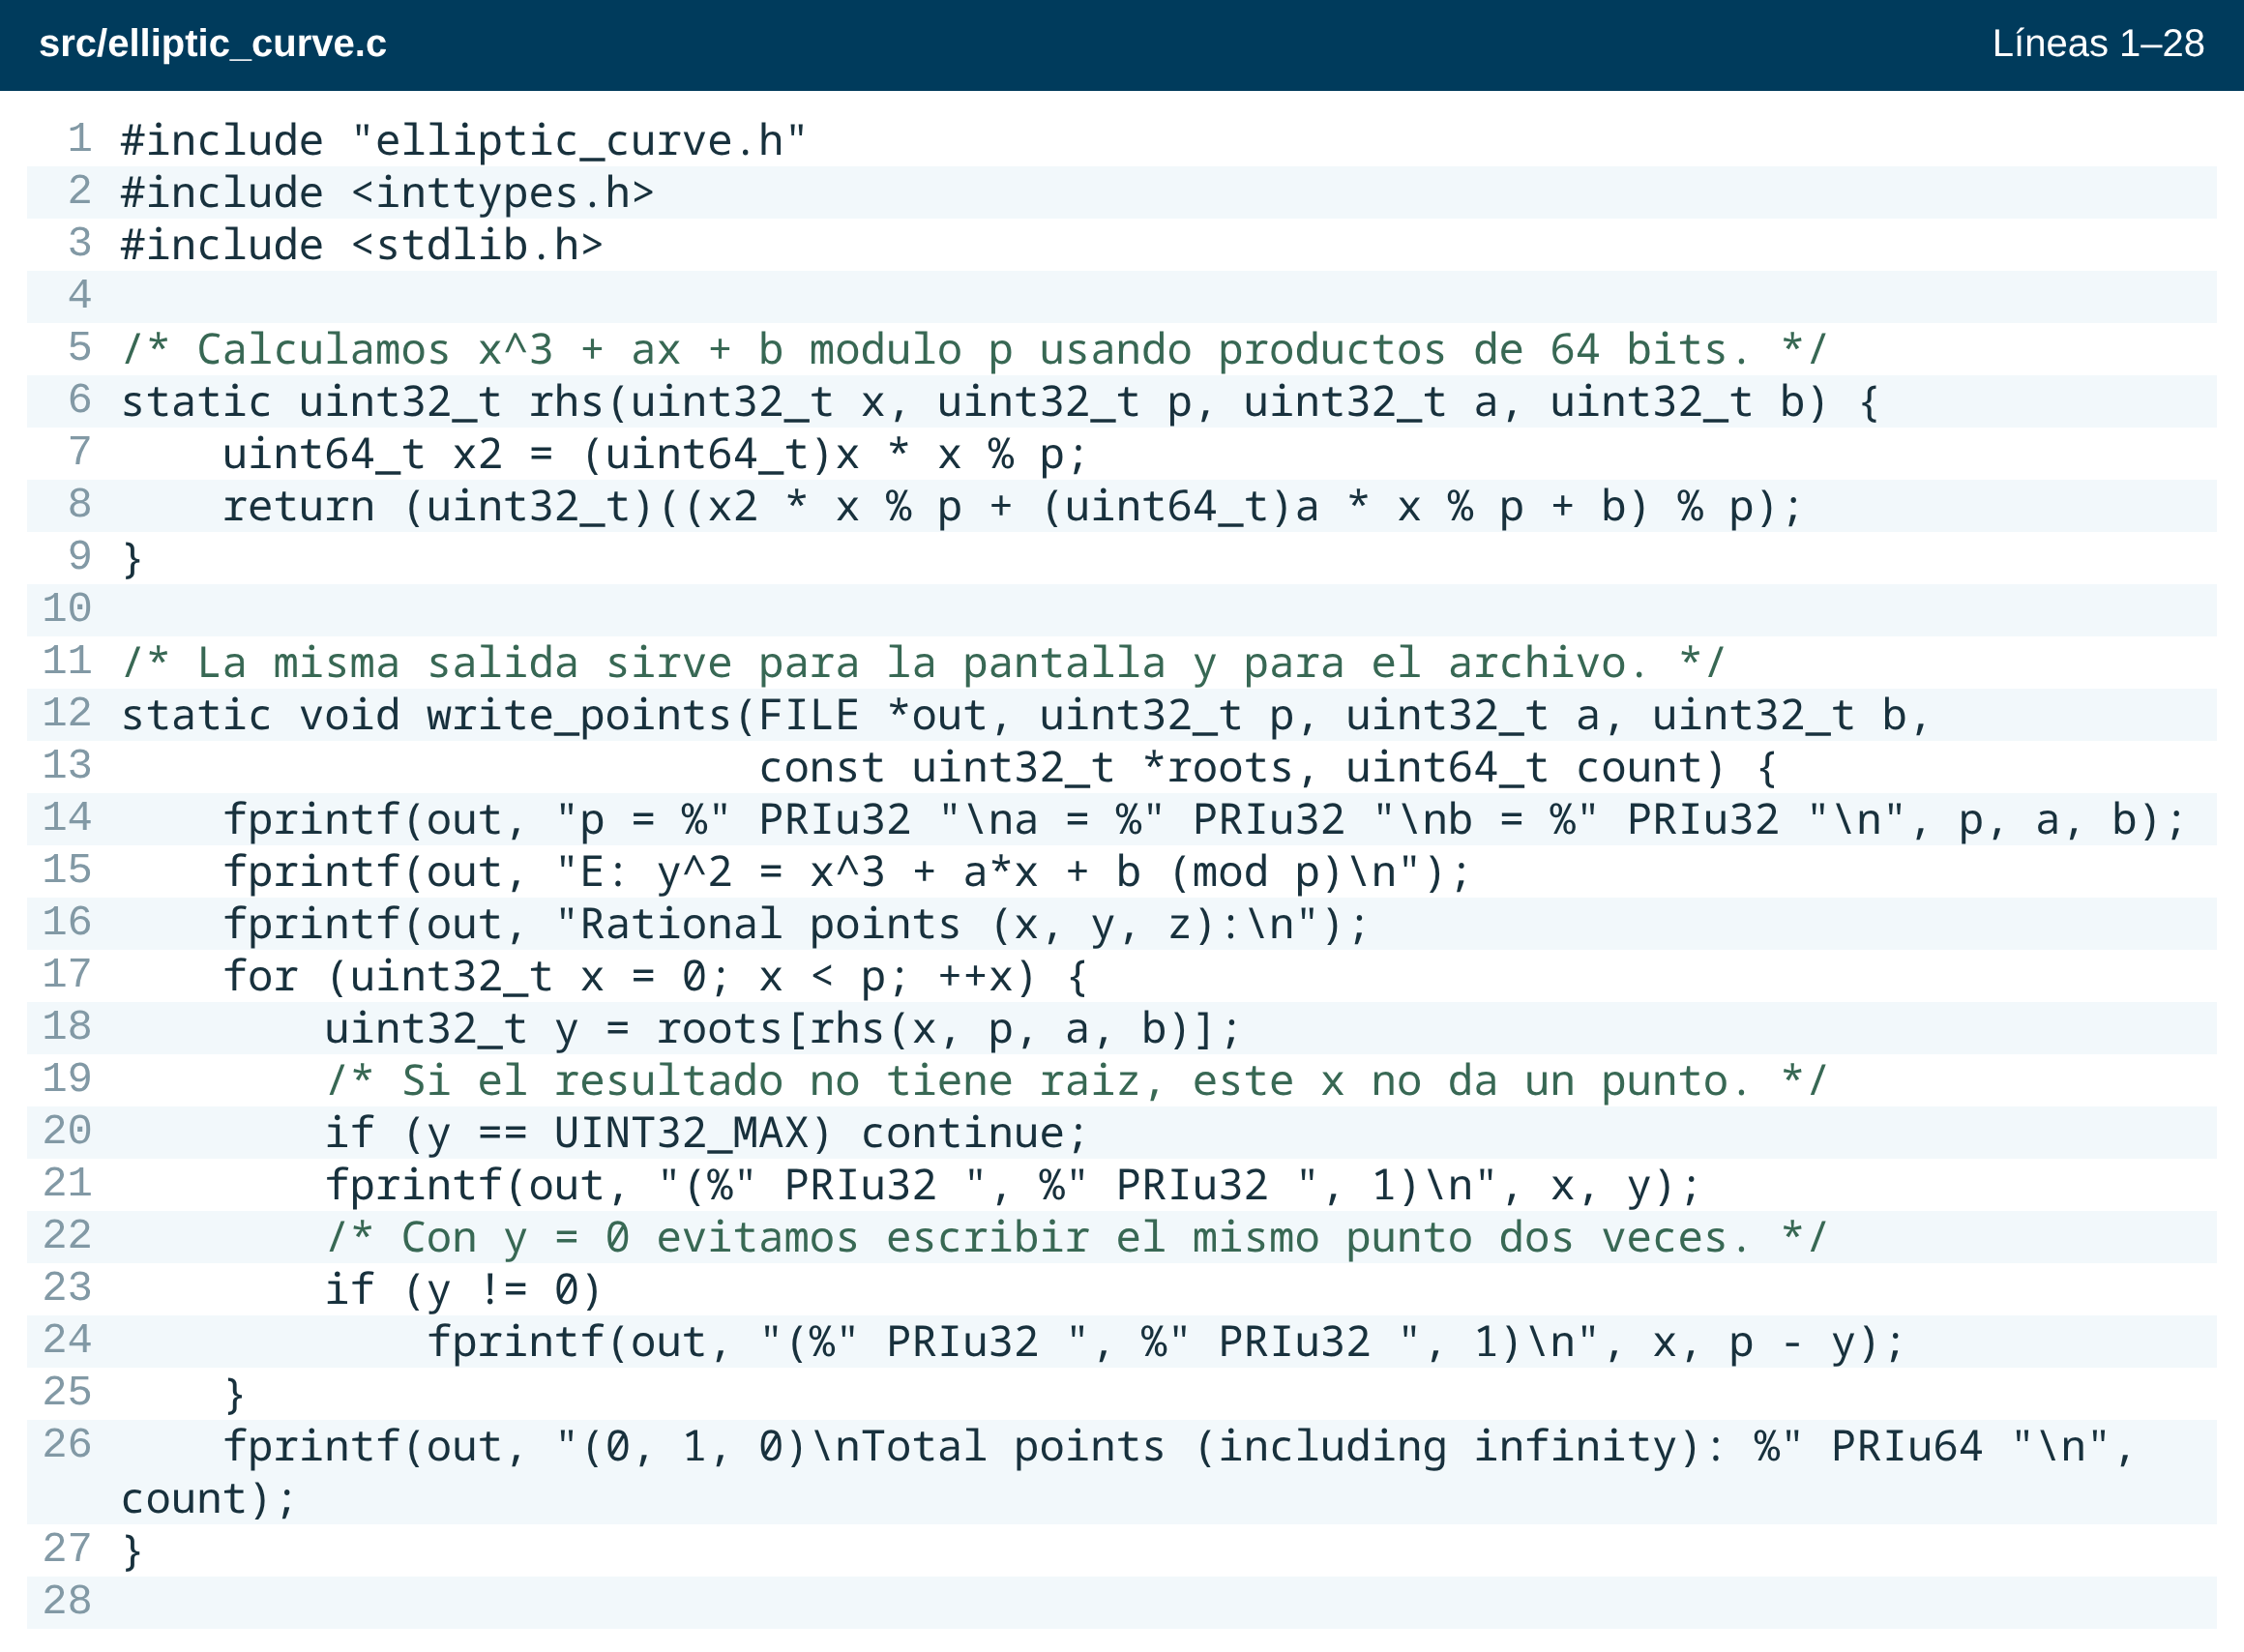
\includegraphics[width=\linewidth,height=0.84\textheight,keepaspectratio]{assets/capturas/final-salida-puntos.png}
\end{center}
\vspace{0.2cm}
\noindent\textbf{Uso de IA.} Se usó ChatGPT/Codex para generar el código de
\texttt{src/} e \texttt{include/}, preparar pruebas y organizar el reporte.
El apoyo se utilizó para construir y comprobar la aritmética con arreglos.
\clearpage
\section*{Conteo y archivo}
\noindent Se cuentan los puntos y se agrega $(0,1,0)$ para el infinito.
\begin{center}
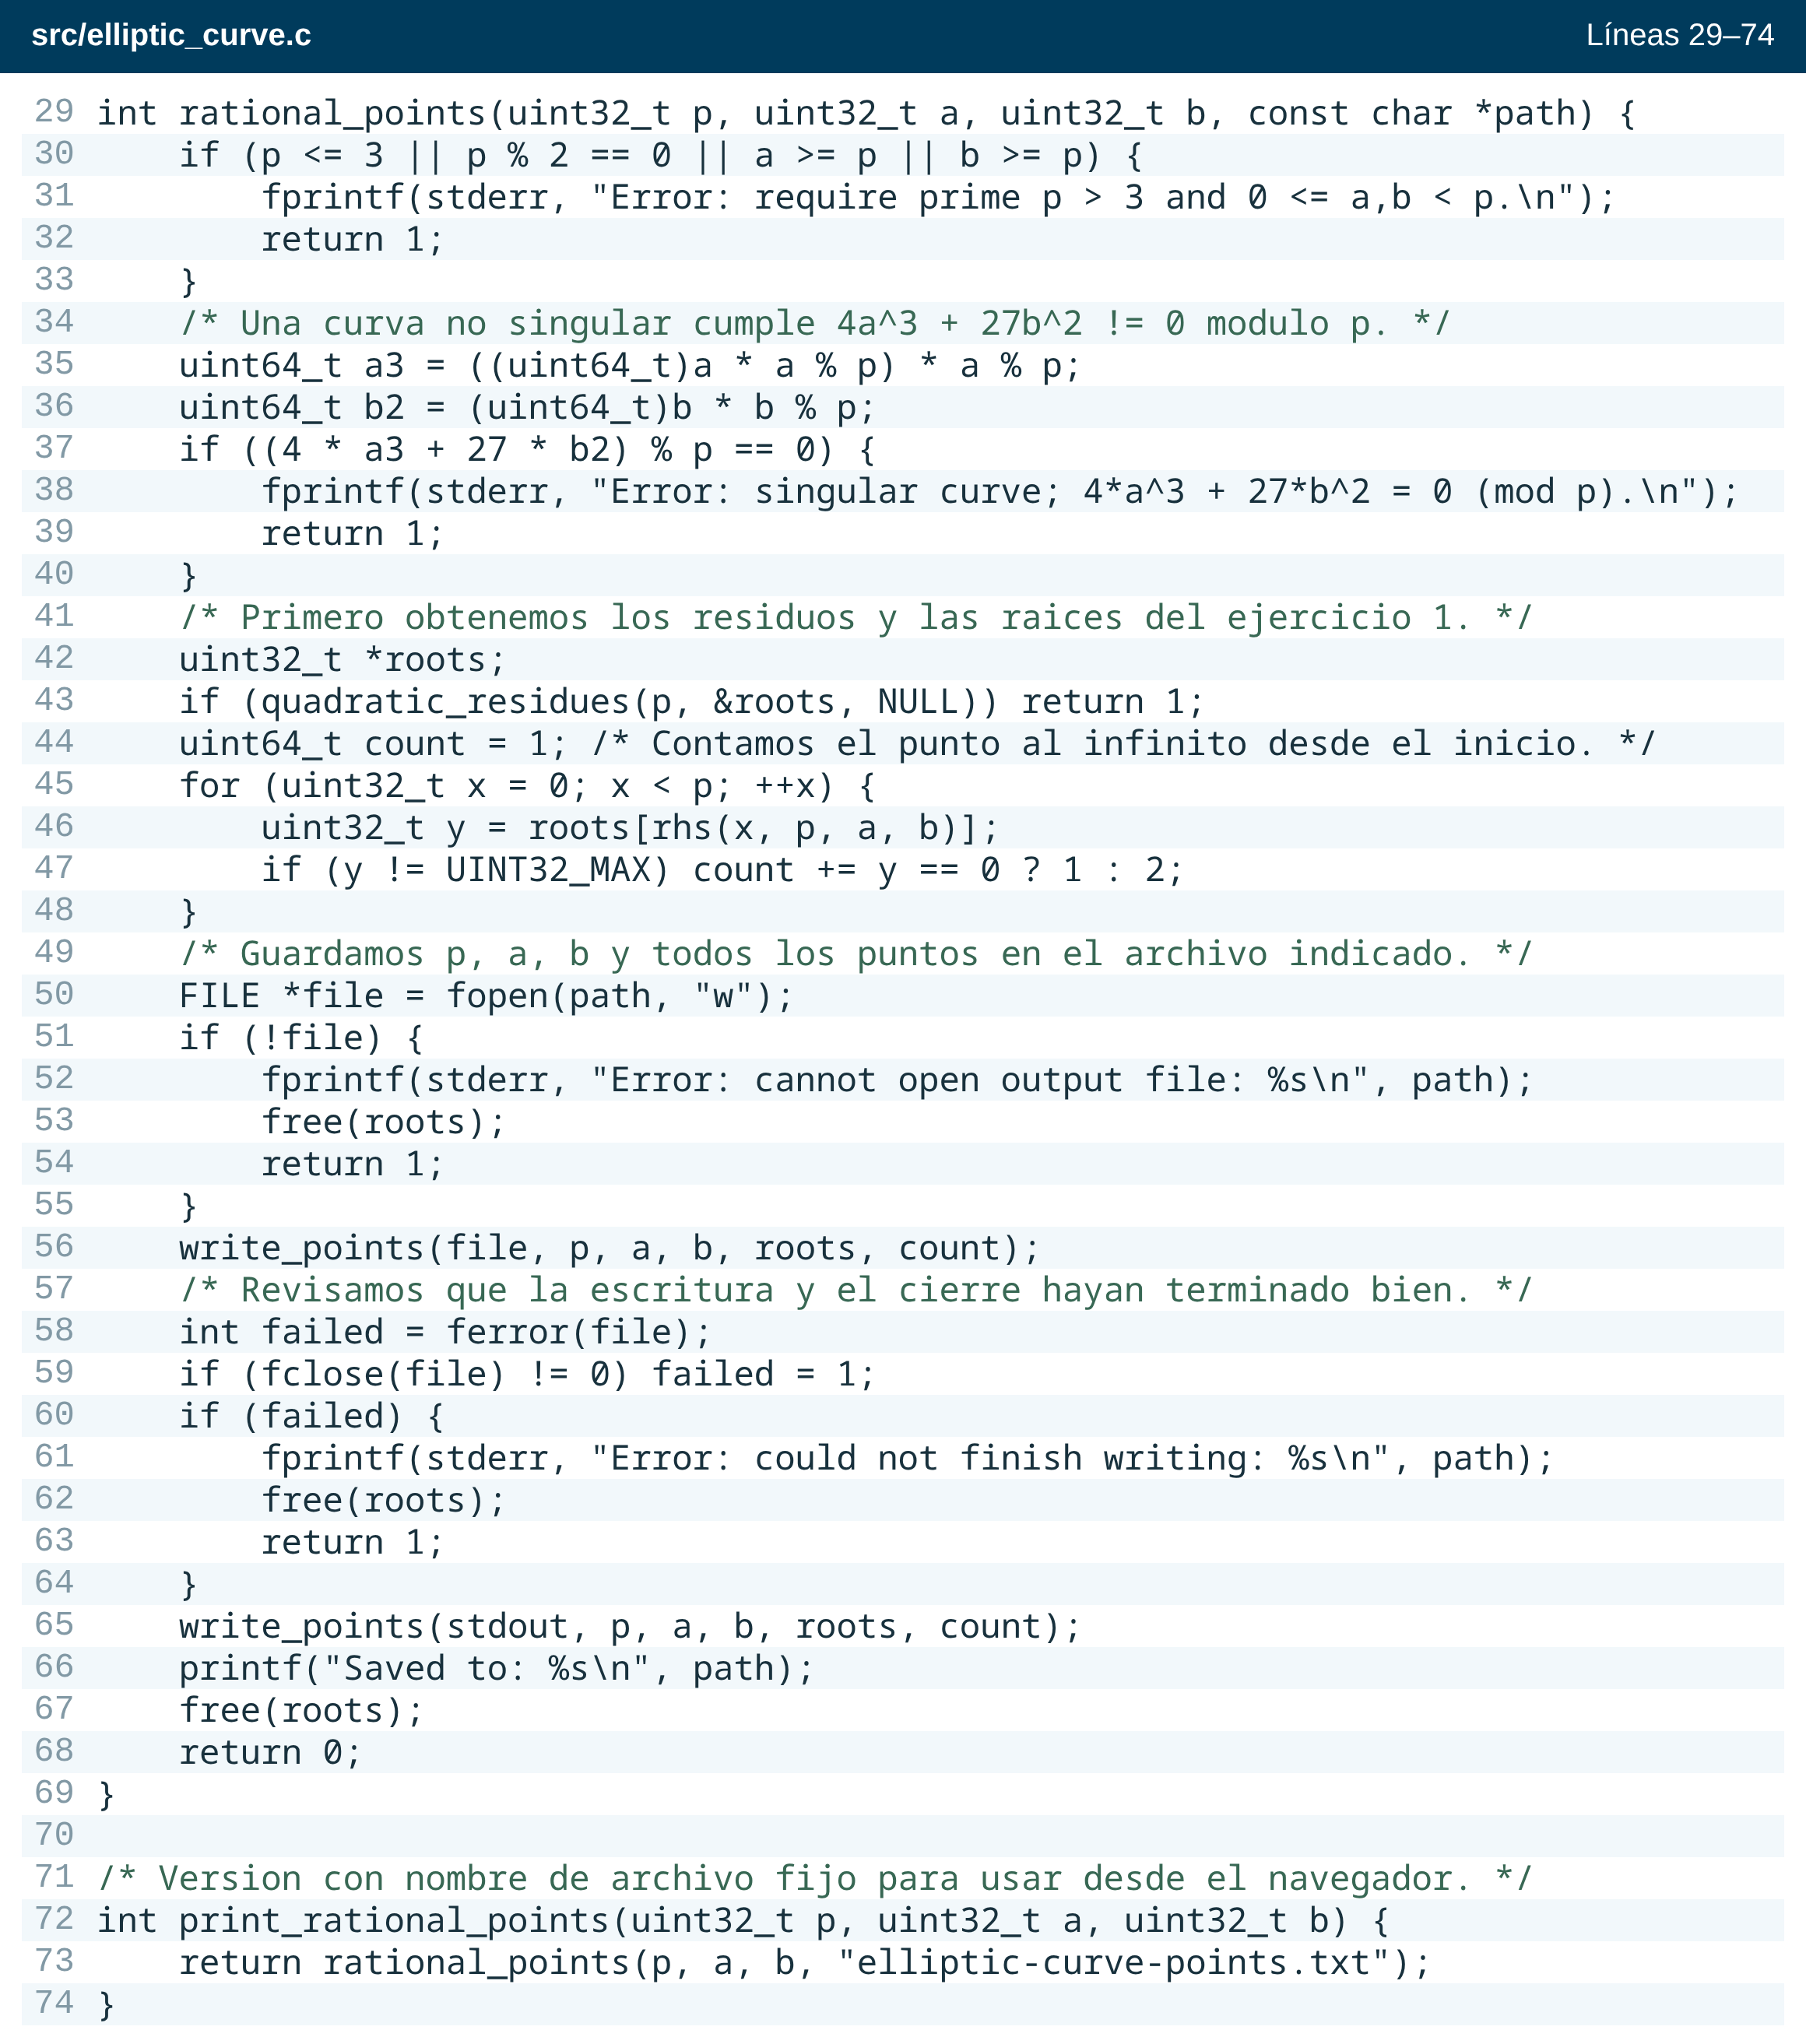
\includegraphics[width=\linewidth,height=0.85\textheight,keepaspectratio]{assets/capturas/final-puntos.png}
\end{center}
\clearpage
\section*{Generación de curvas}
\noindent Se genera un candidato de $n$ bits y se busca $4a^3+27b^2\not\equiv0\pmod p$.
\begin{center}
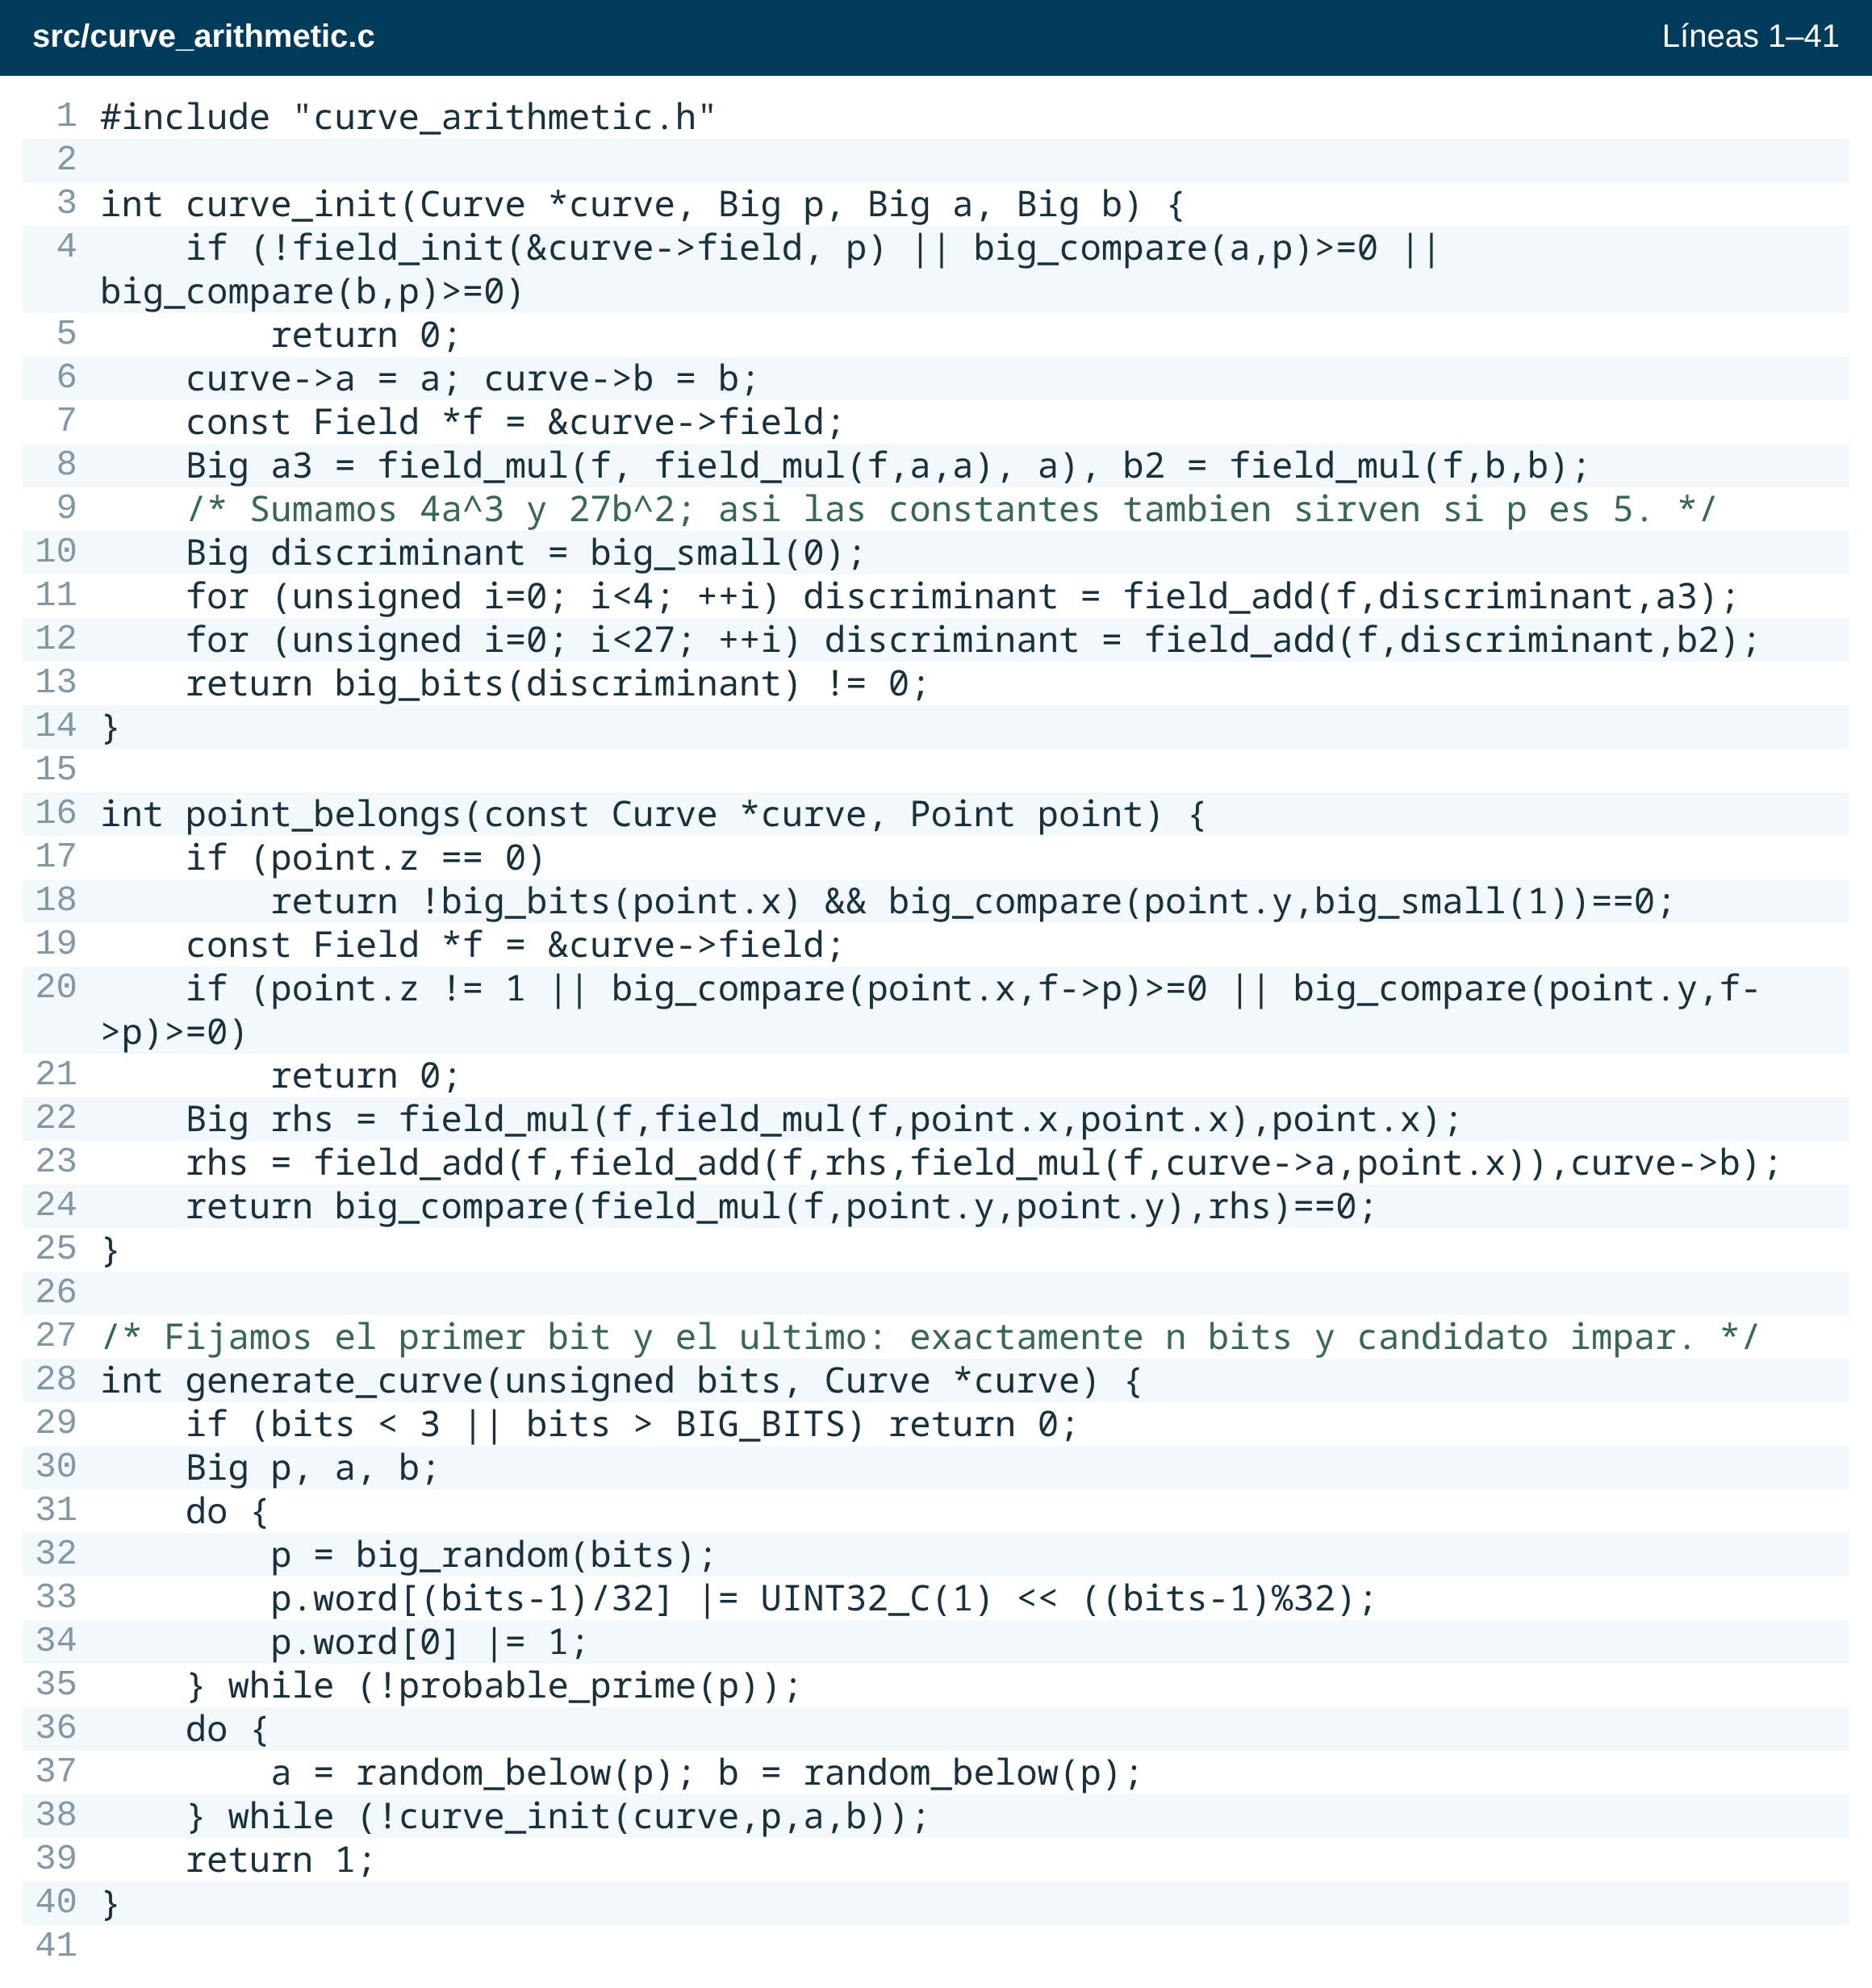
\includegraphics[width=\linewidth,height=0.81\textheight,keepaspectratio]{assets/capturas/final-generacion.png}
\end{center}
\noindent\small C17 estándar. Los enteros usan arreglos de 32 bits.
Miller--Rabin hace 32 rondas: el resultado es un primo probable.
\texttt{rand} se usa para la práctica, no para generar claves de uso real.
\clearpage
\section*{Suma y duplicación}
\noindent Se revisan los puntos, se calcula la pendiente y se obtiene el resultado módulo $p$.
\begin{center}
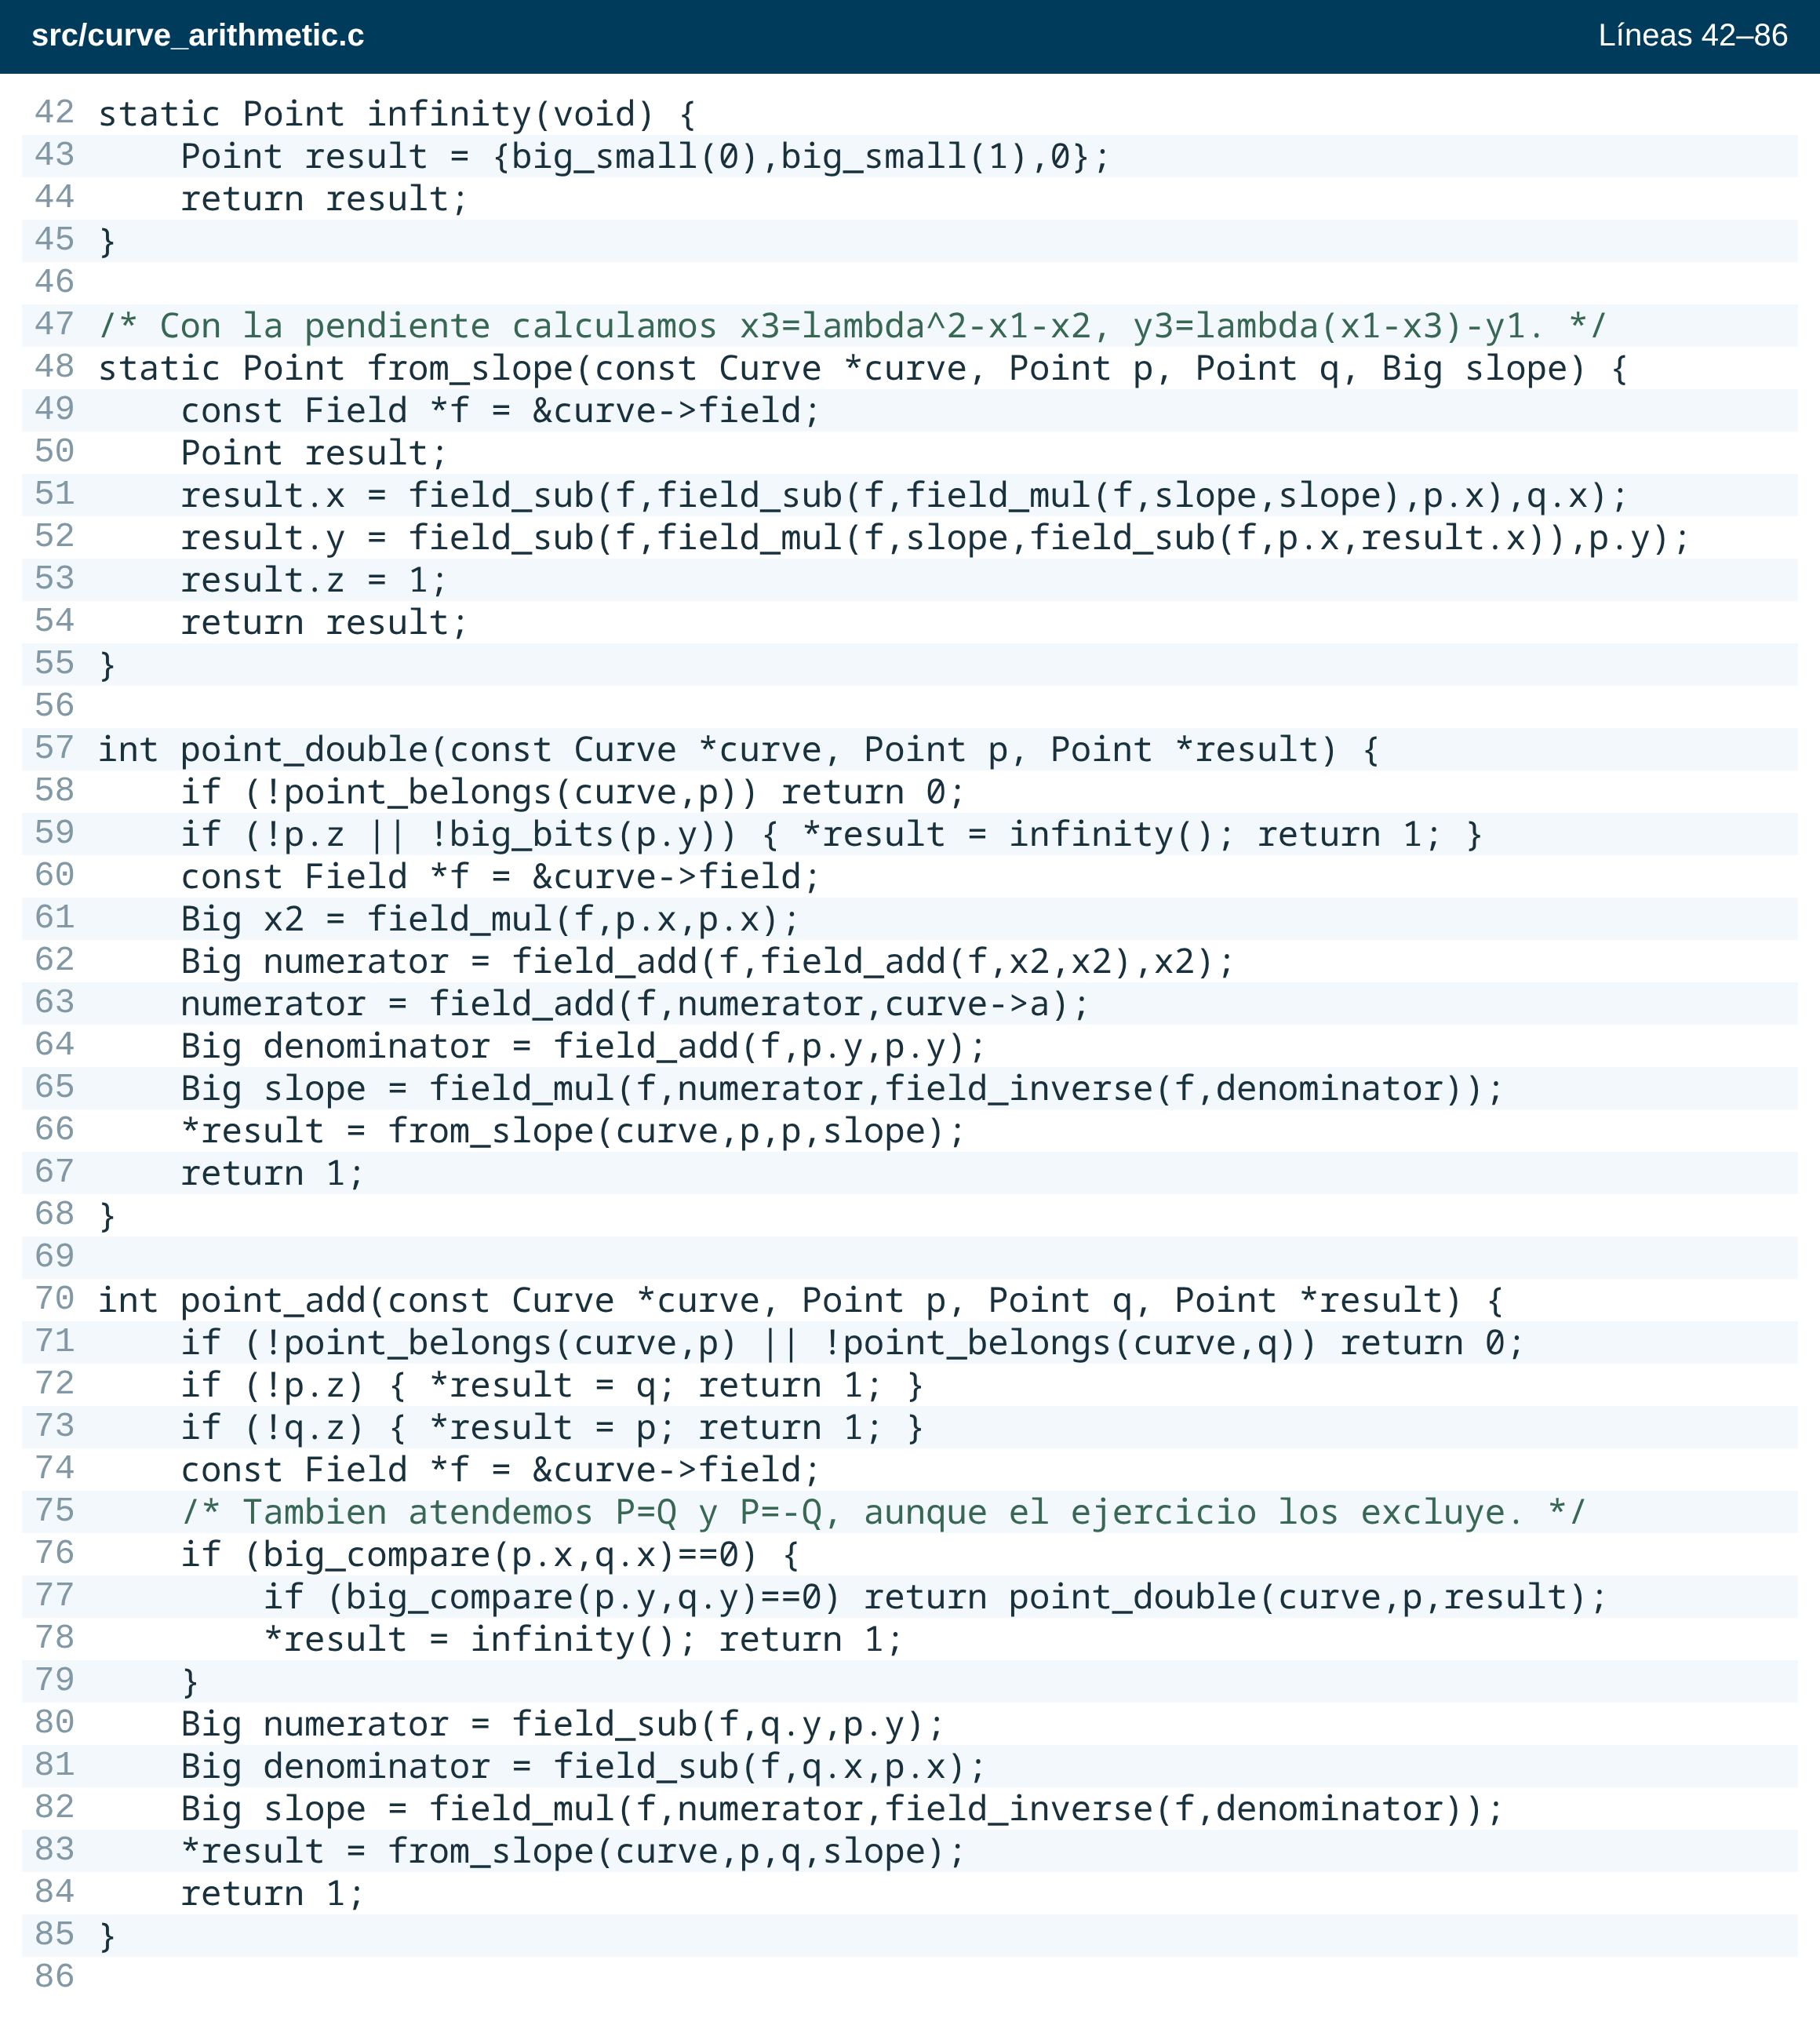
\includegraphics[width=\linewidth,height=0.85\textheight,keepaspectratio]{assets/capturas/final-aritmetica.png}
\end{center}
\clearpage
\section*{Captura de consola}
\begin{center}
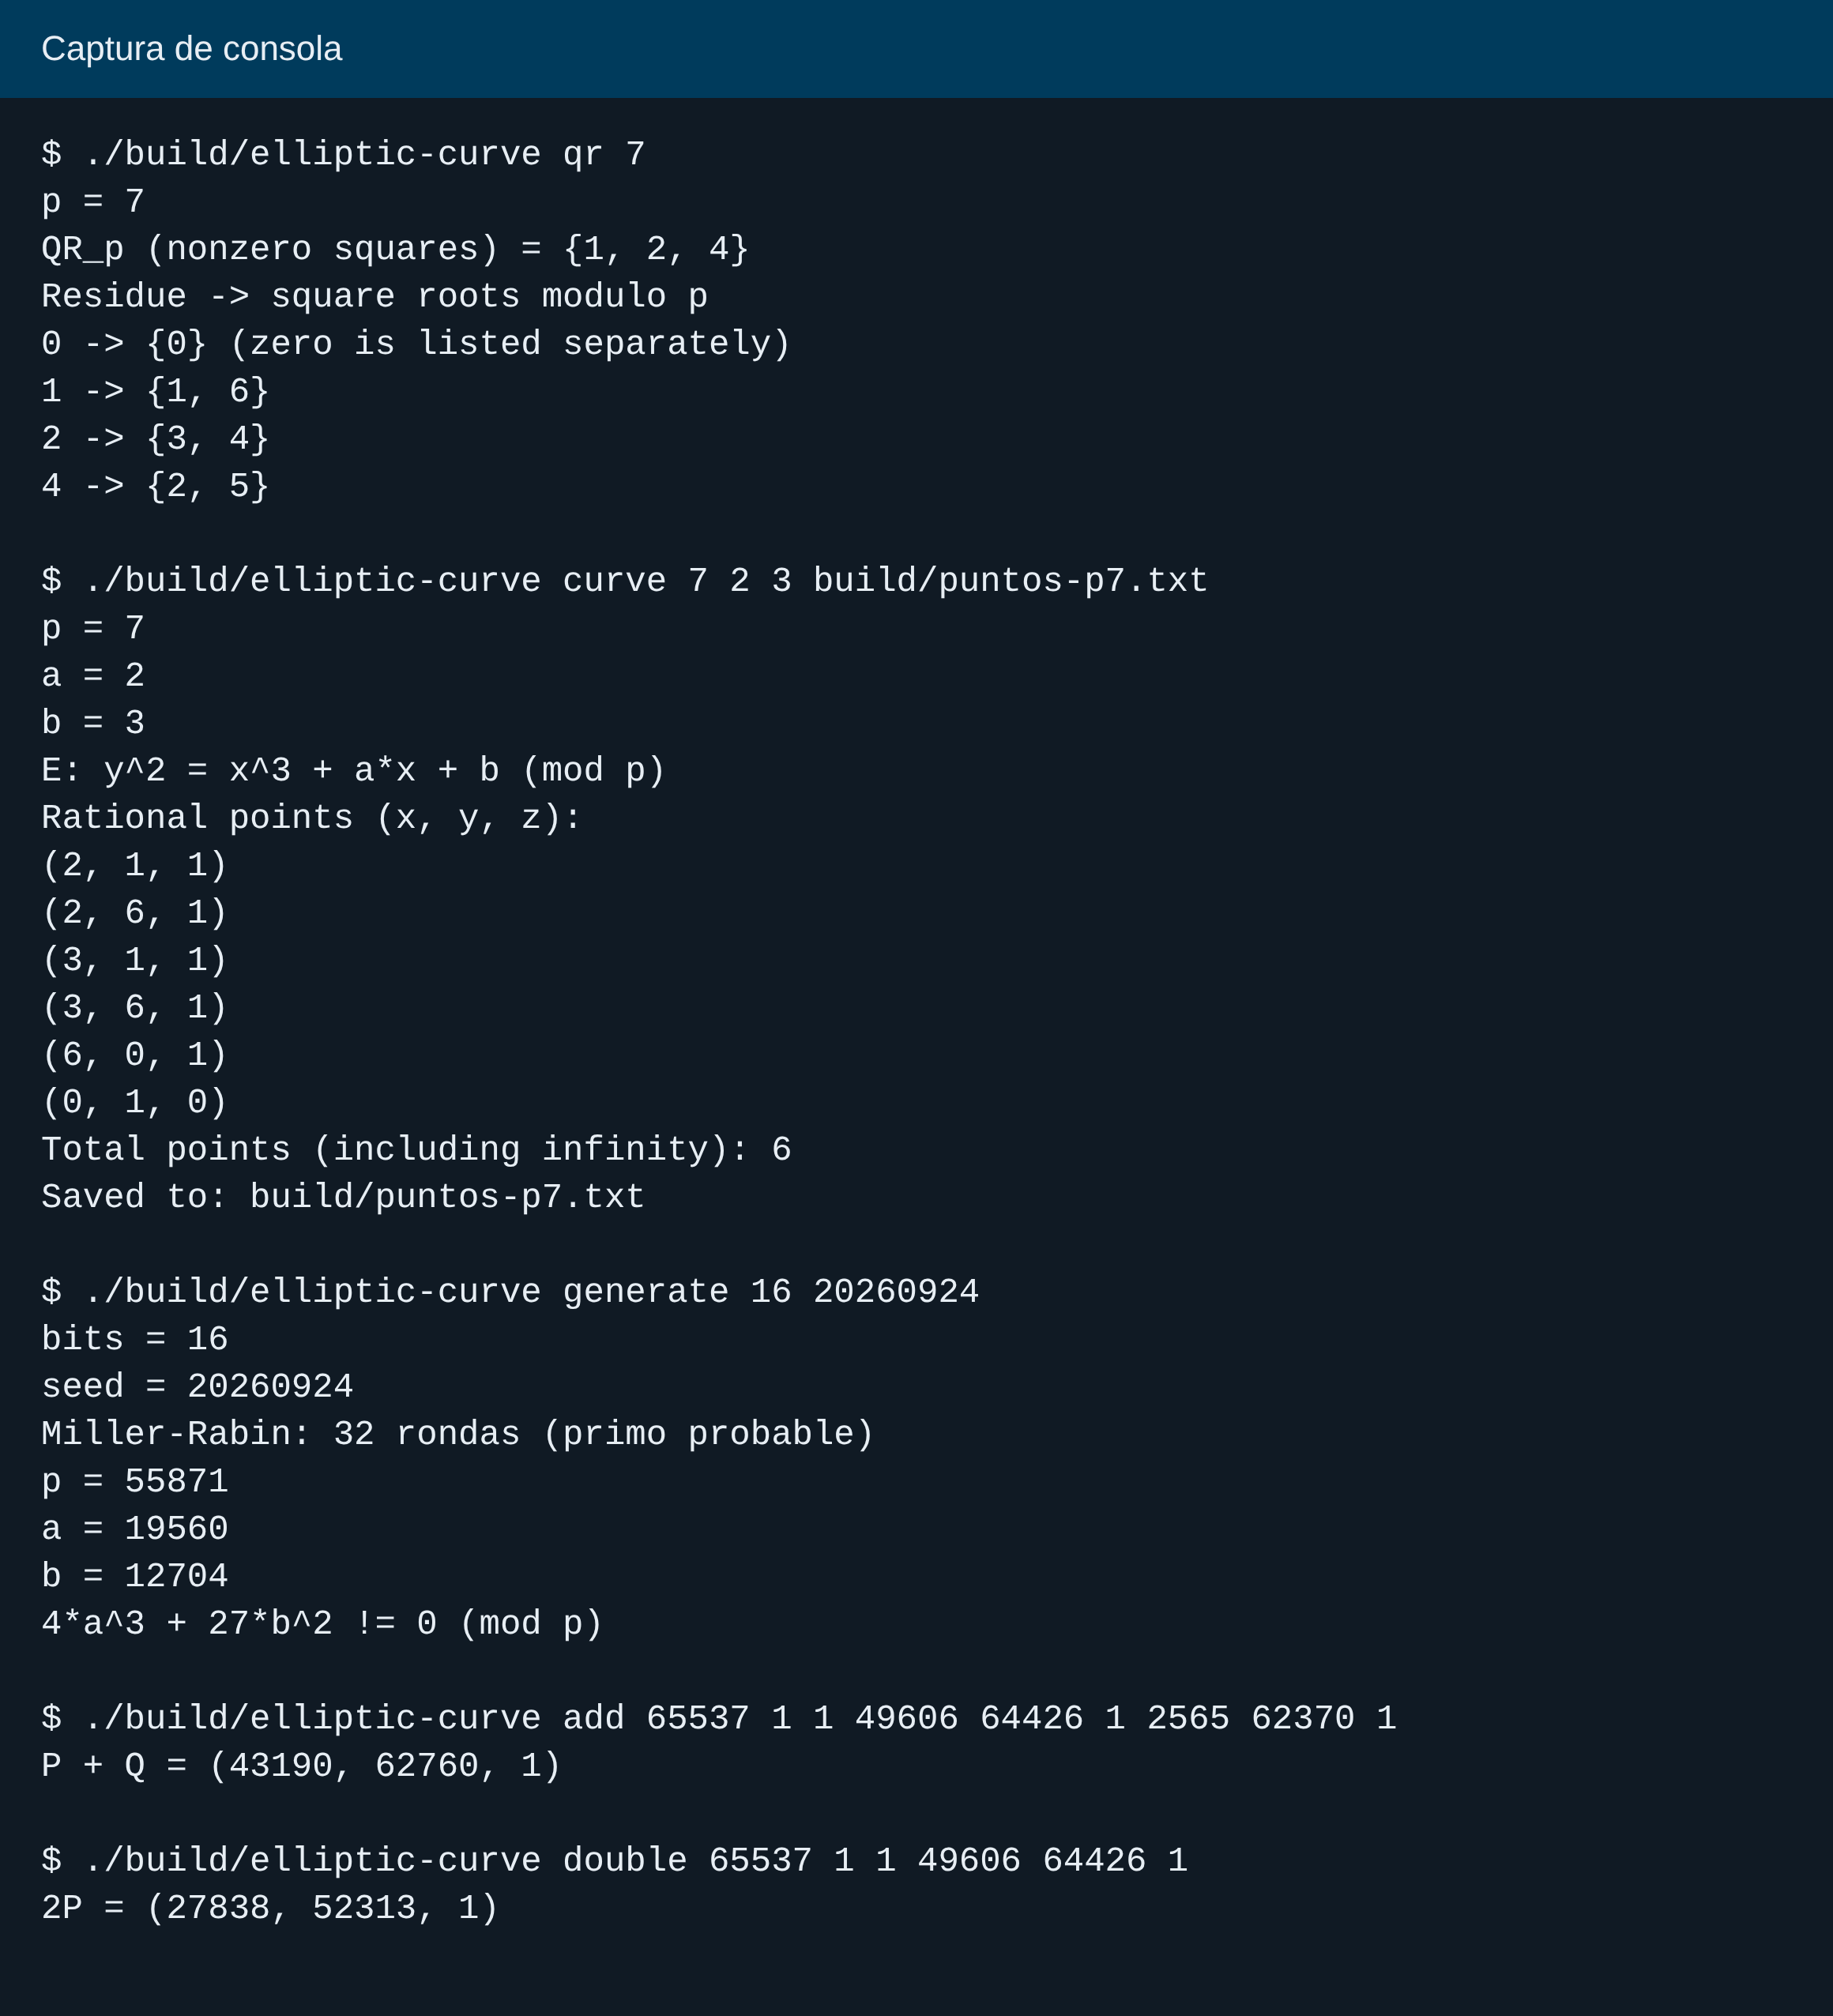
\includegraphics[width=\linewidth,height=0.88\textheight,keepaspectratio]{assets/capturas/final-consola.png}
\end{center}
\clearpage
\section*{3.1. Gráficas de puntos racionales}
\noindent Se graficaron los archivos \texttt{puntos-17.txt}, \texttt{puntos-97.txt} y
\texttt{puntos-101.txt}. El infinito se cuenta, pero no se dibuja en el plano.
\begin{center}
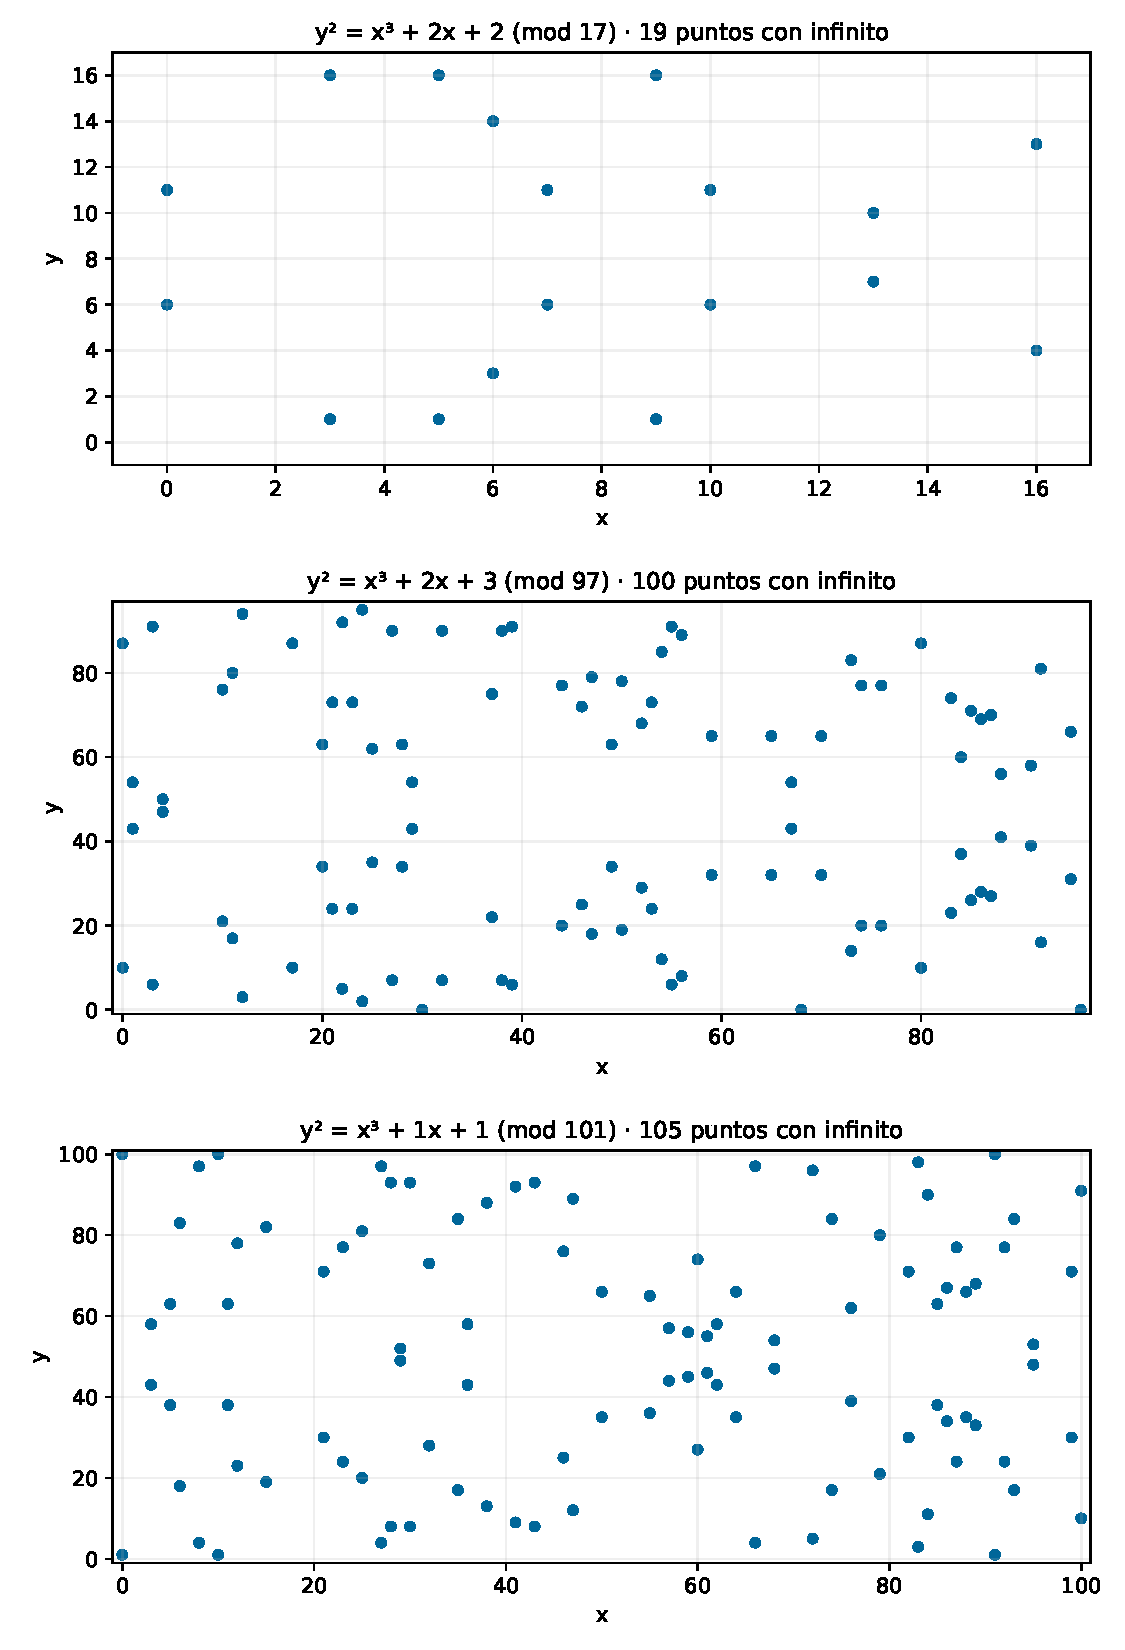
\includegraphics[width=\linewidth,height=0.85\textheight,keepaspectratio]{assets/resultados/graficas.pdf}
\end{center}
\clearpage
\section*{3.2. Curvas de 16, 32, 64 y 512 bits}
\noindent En todos los casos: $y^2=x^3+ax+b\bmod p$ y $4a^3+27b^2\not\equiv0\pmod p$.
\begin{center}
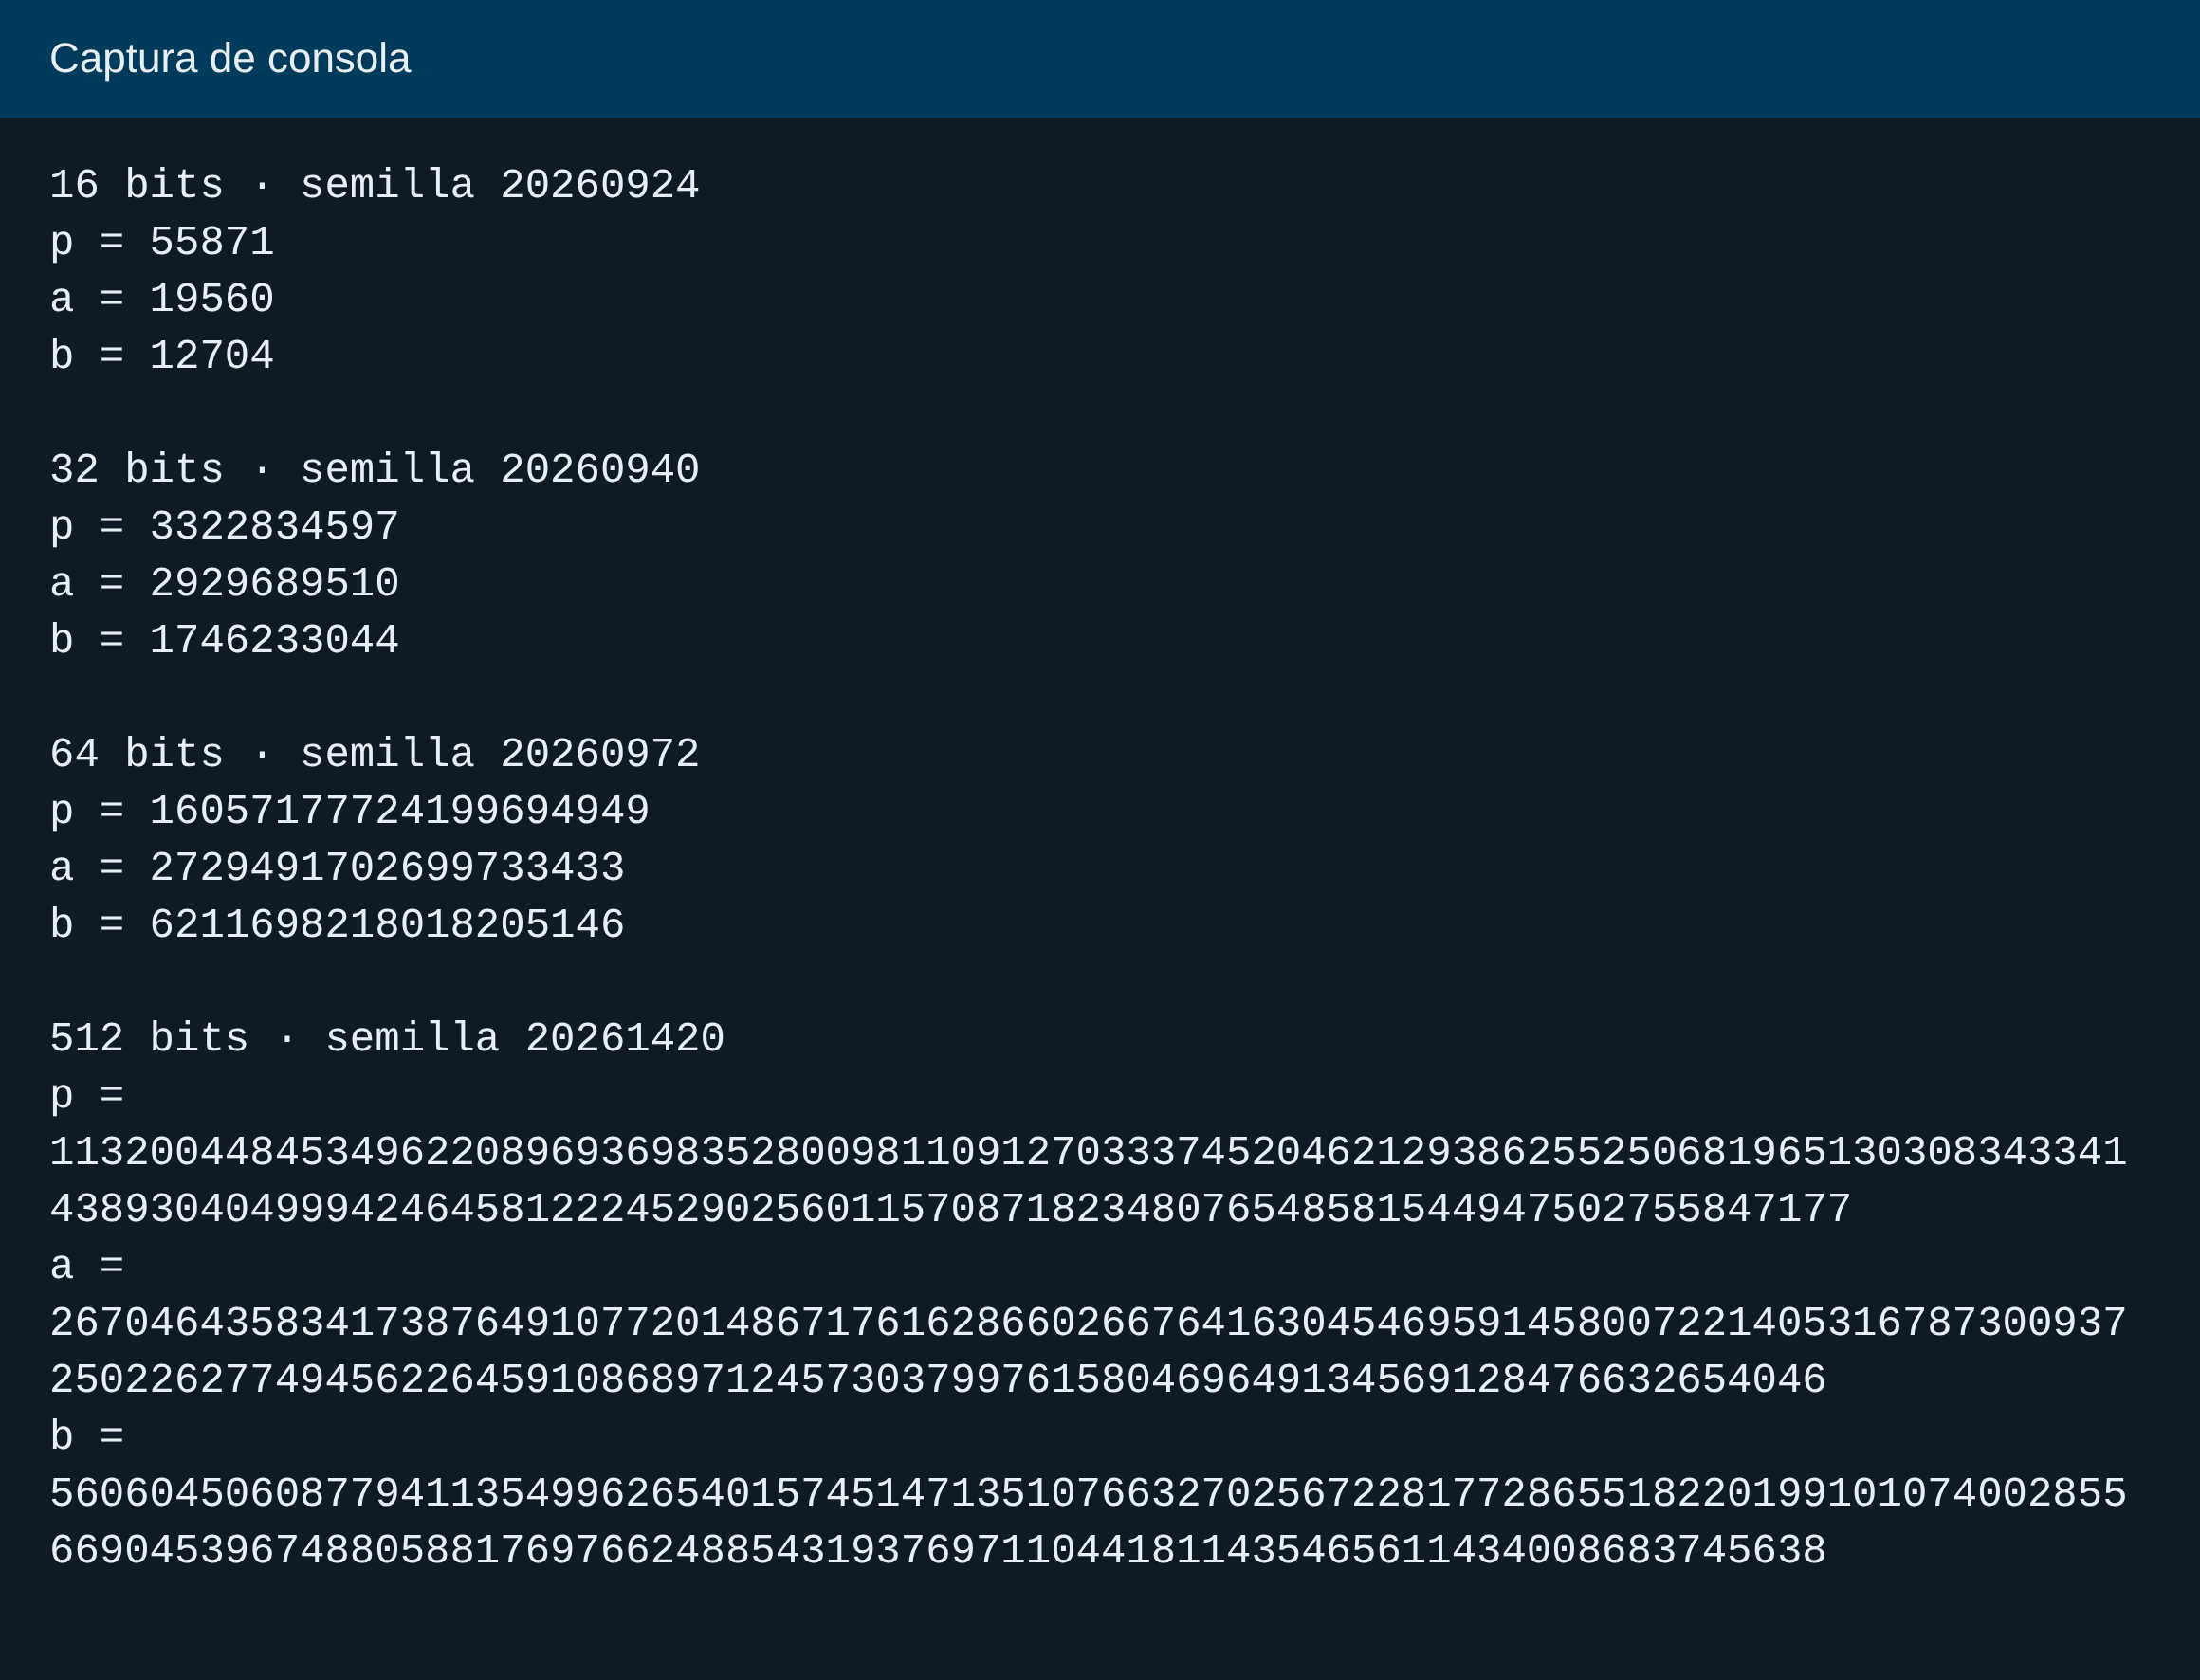
\includegraphics[width=\linewidth,height=0.85\textheight,keepaspectratio]{assets/capturas/final-primos-pequenas.png}
\end{center}
\clearpage
\section*{3.2. Curvas de 1024 y 2048 bits}
\begin{center}
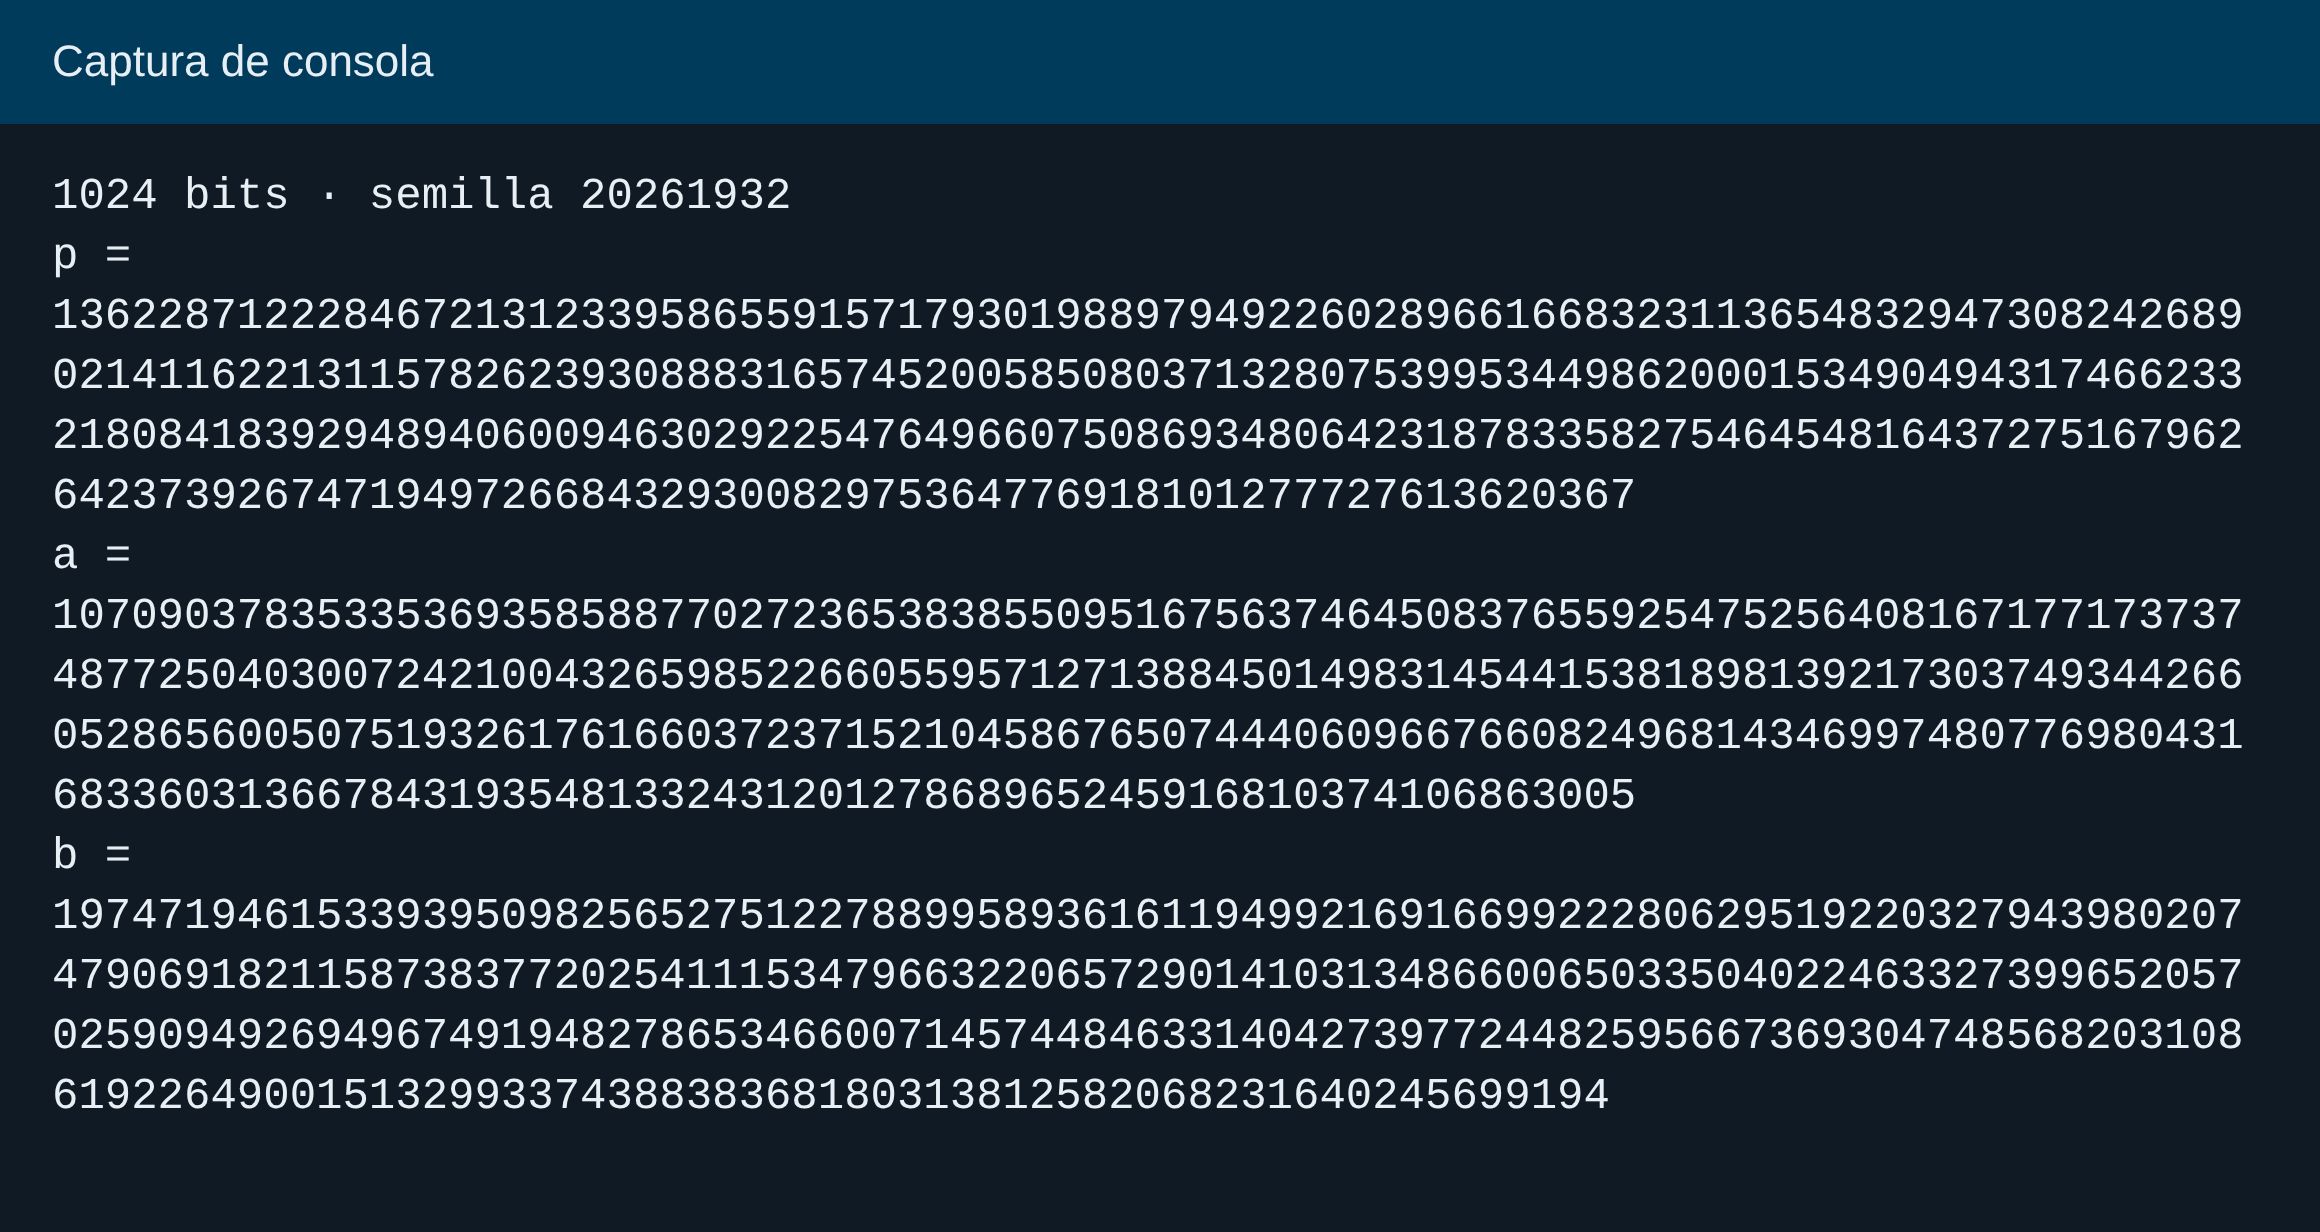
\includegraphics[width=0.90\linewidth]{assets/capturas/final-primos-1024.png}
\par\vspace{0.25cm}
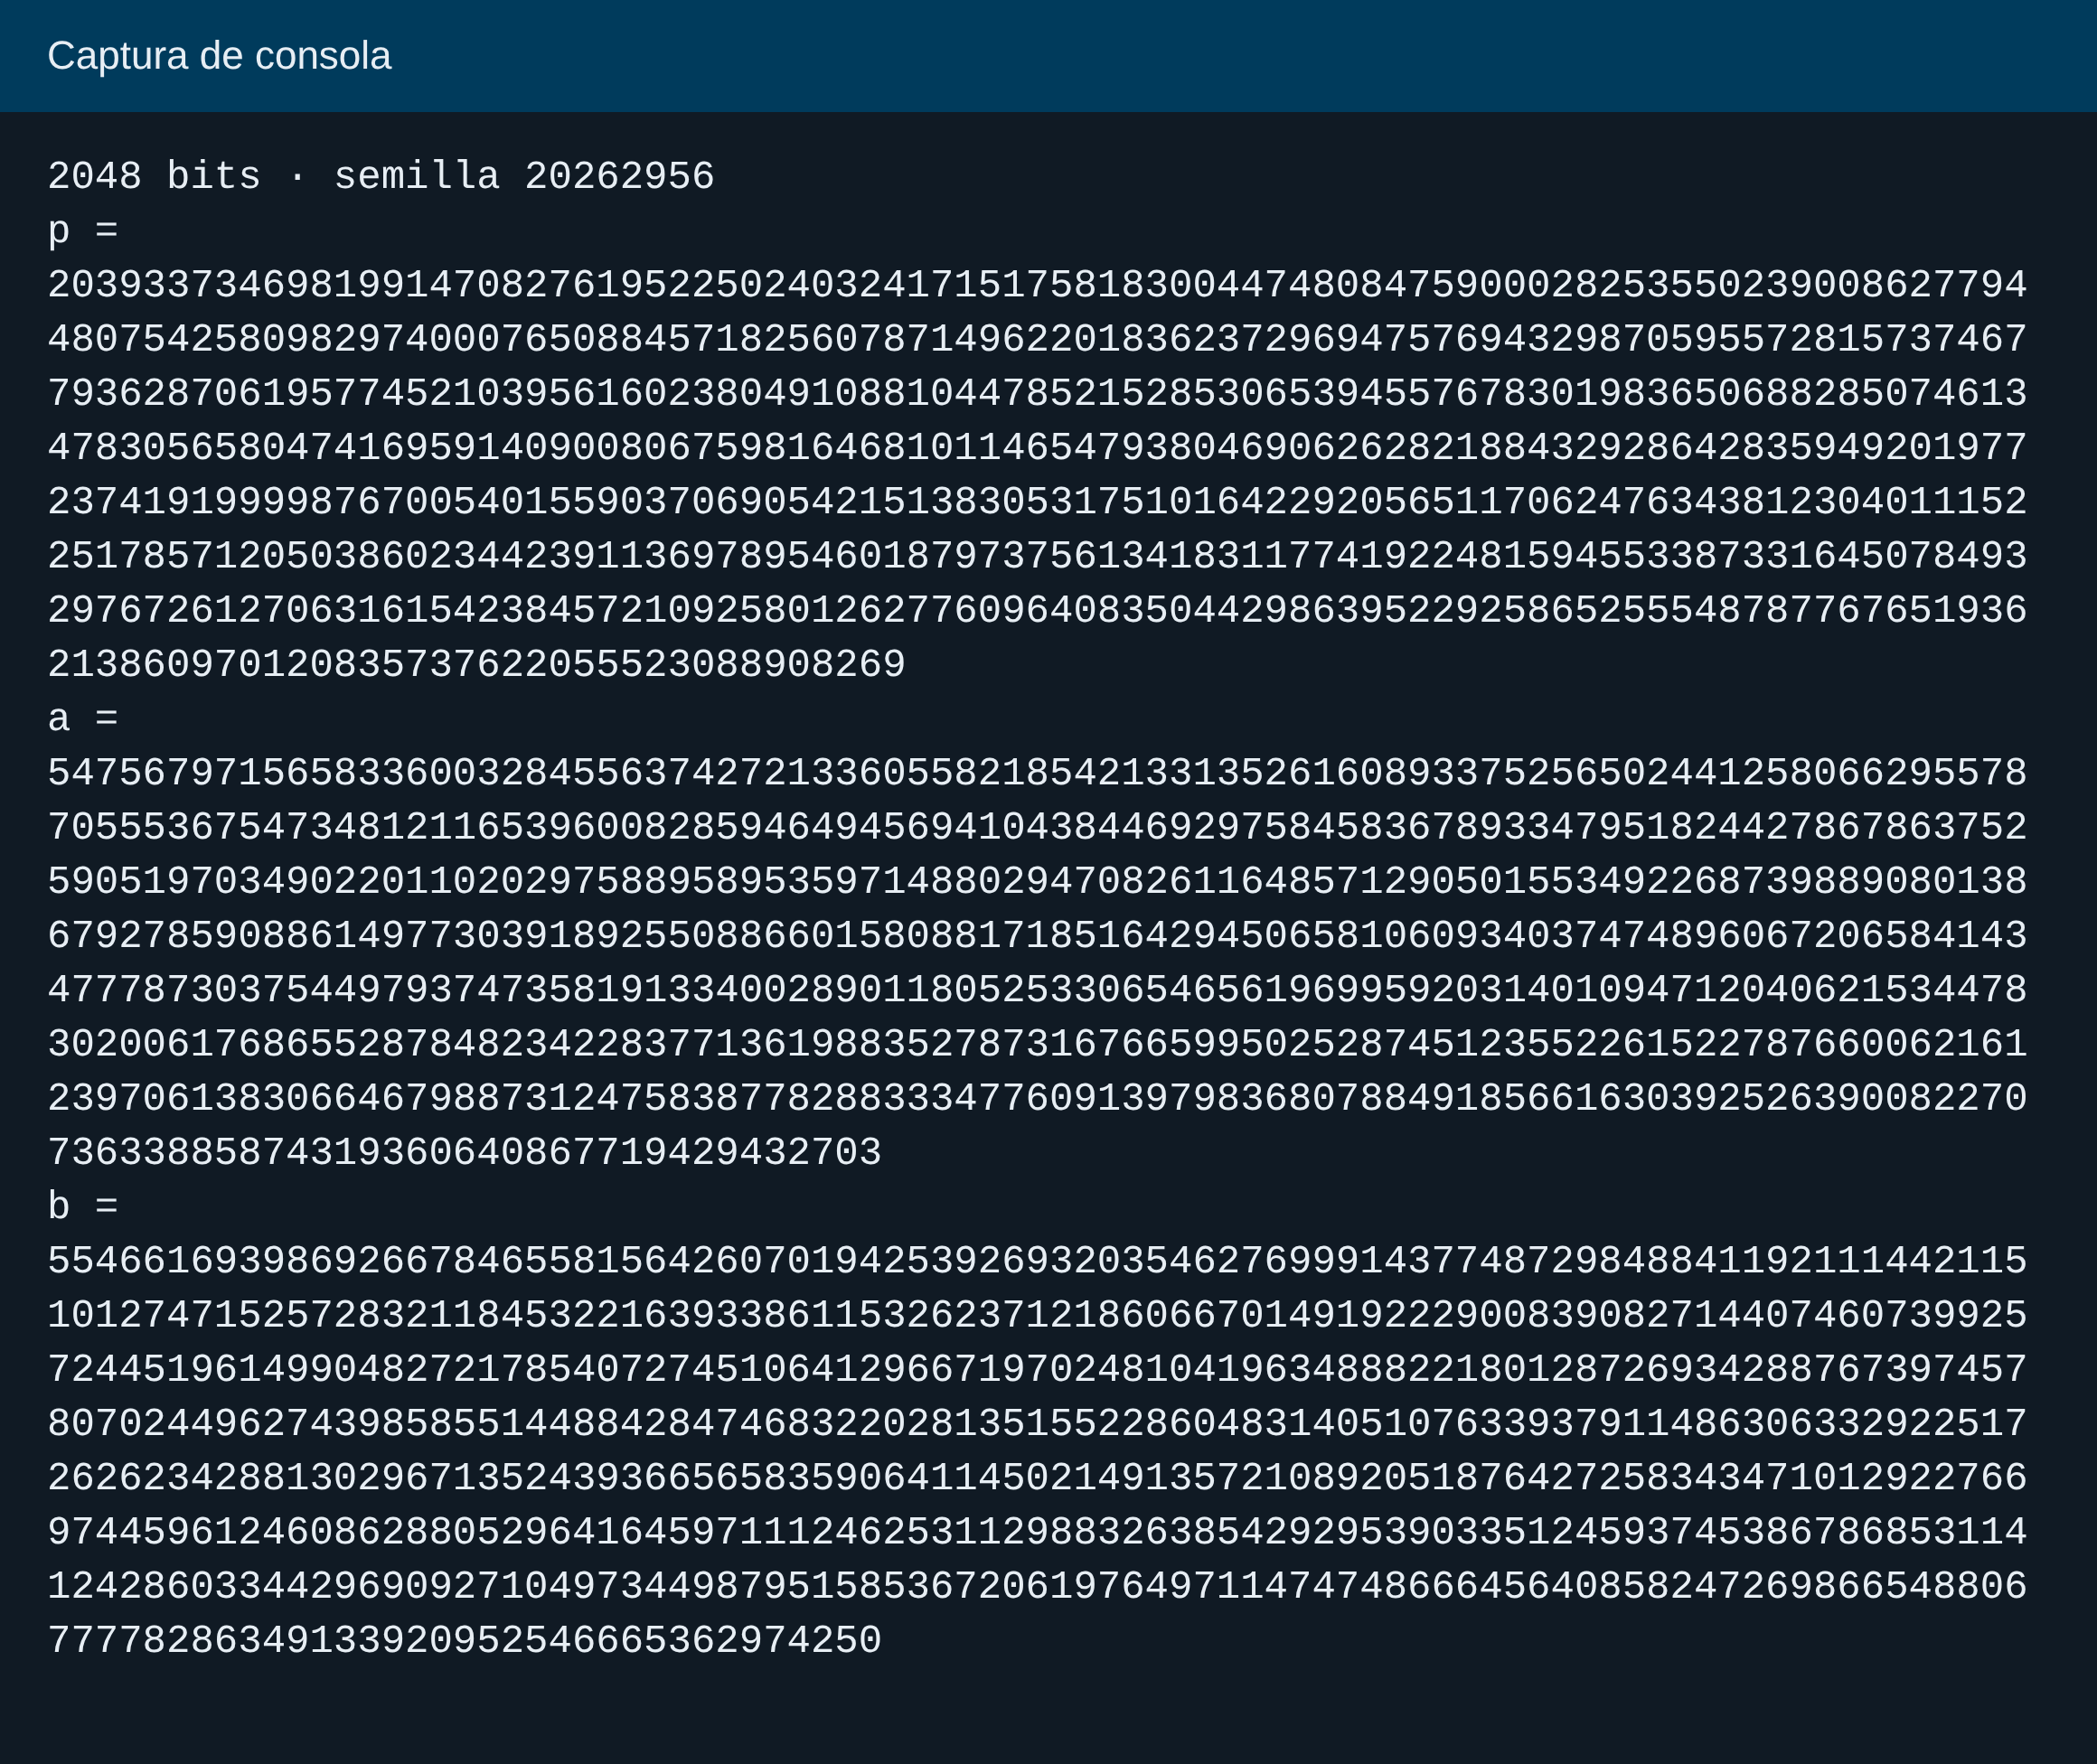
\includegraphics[width=0.90\linewidth]{assets/capturas/final-primos-2048.png}
\end{center}
\clearpage
\section*{3.3. Resultados de las operaciones}
\noindent Se usaron los puntos $P$ y $Q$ de los cuatro incisos del enunciado.
\begin{center}
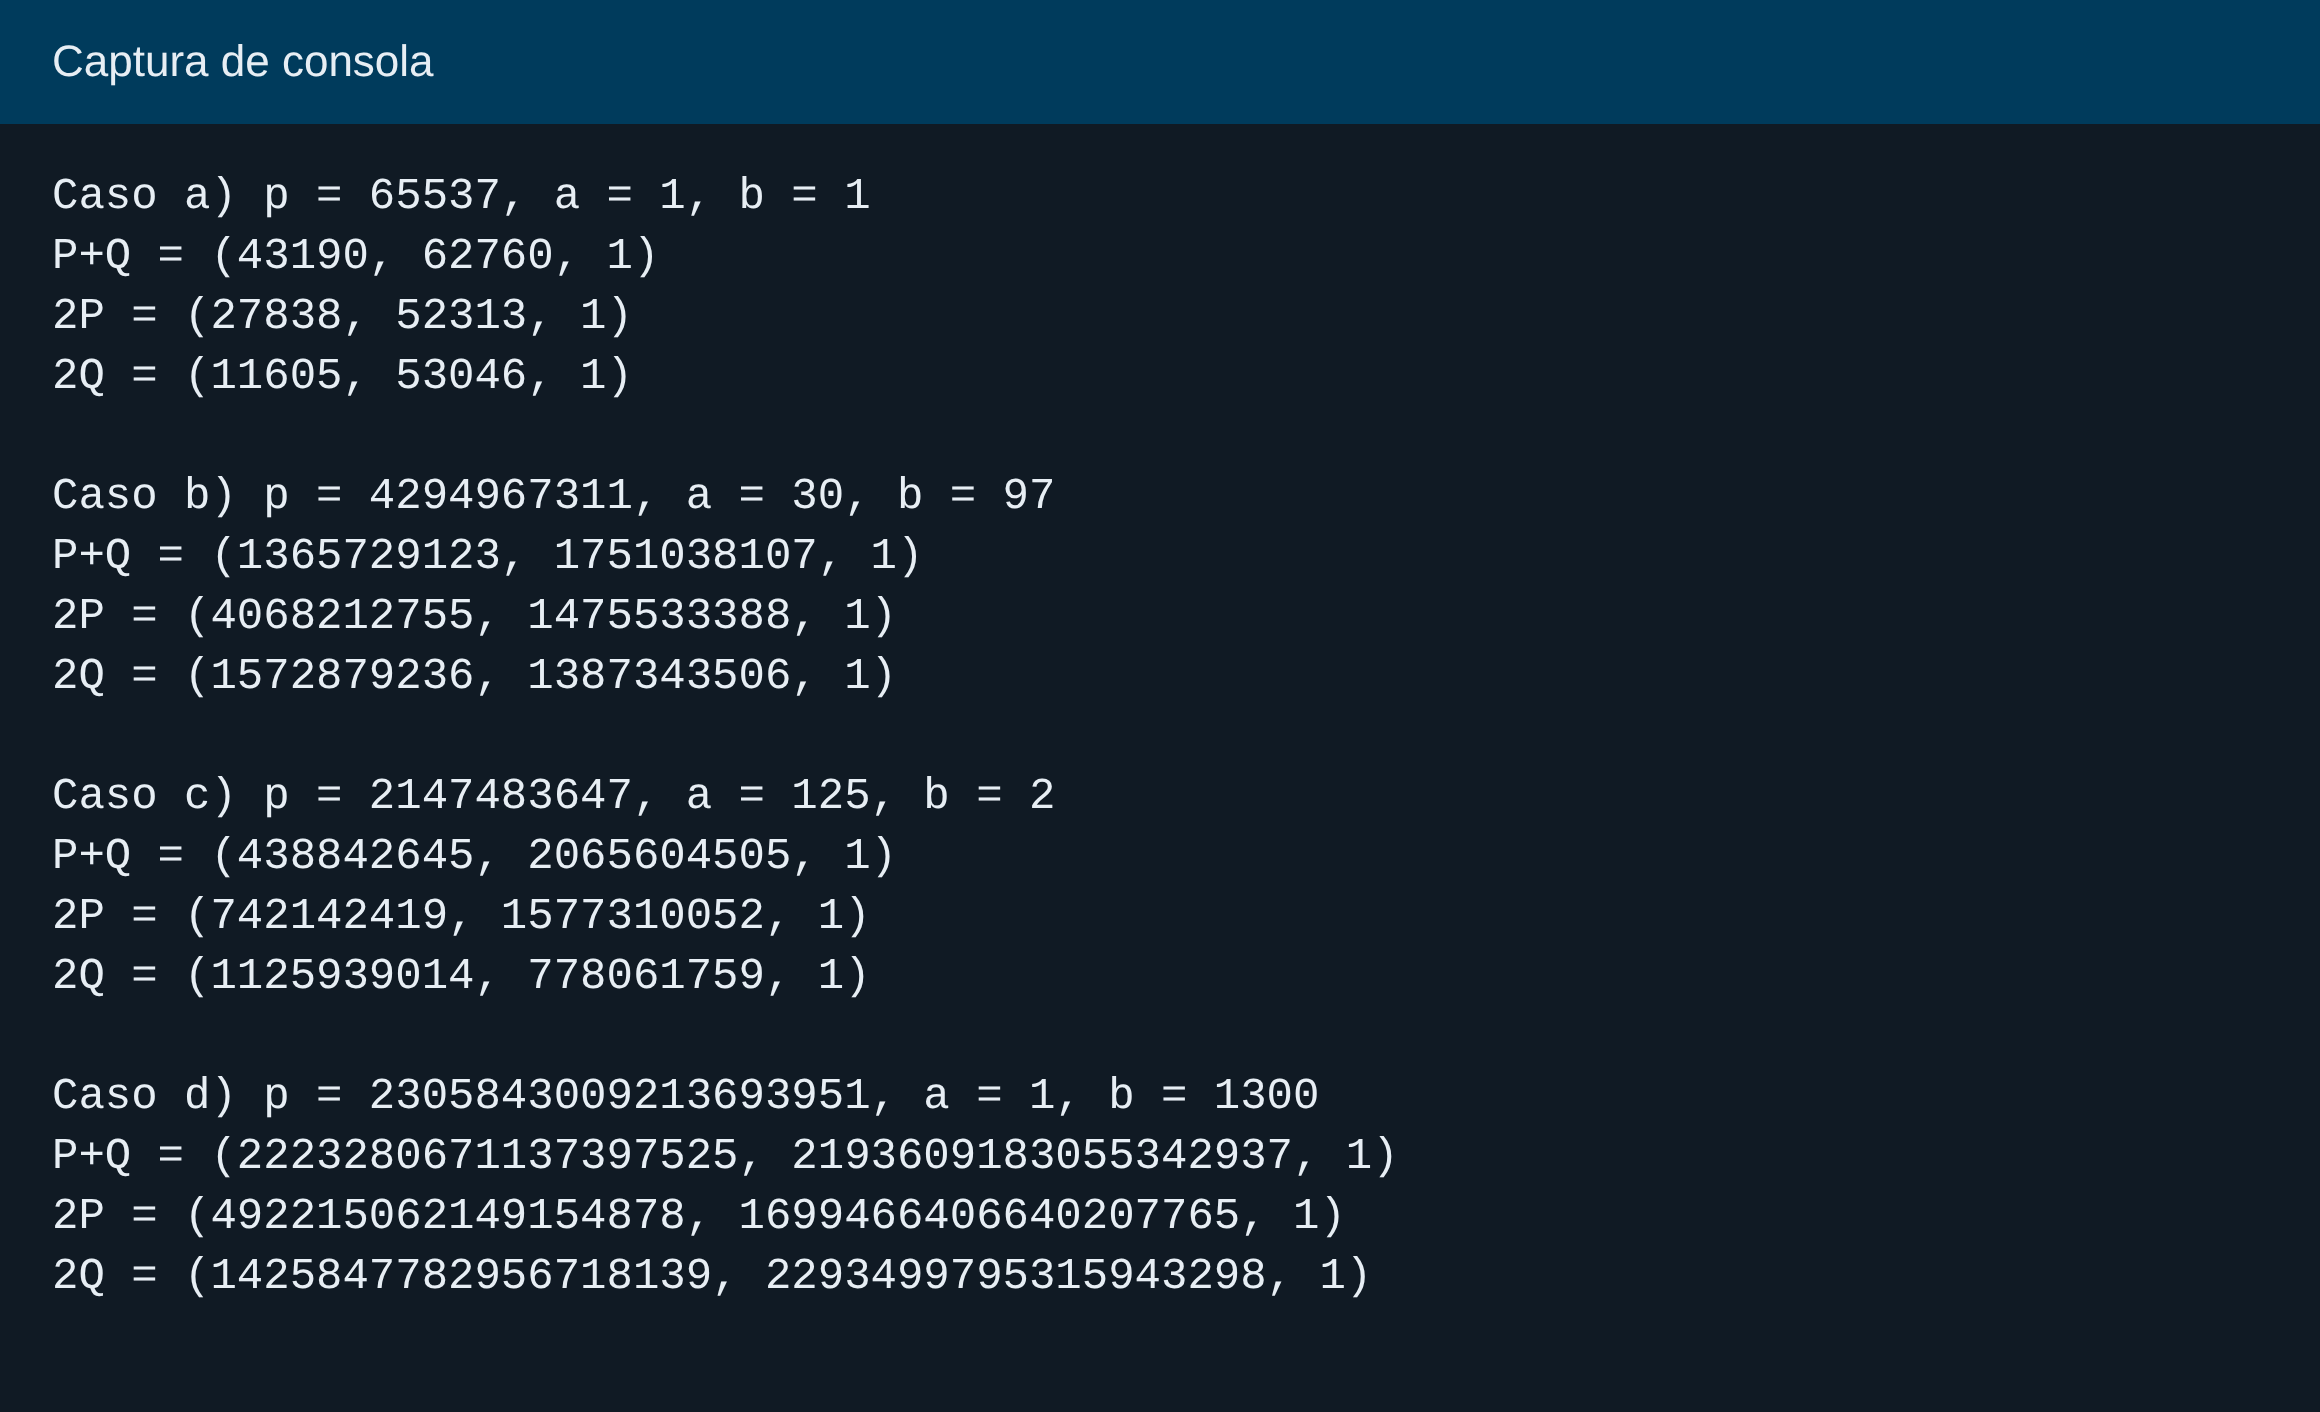
\includegraphics[width=\linewidth,height=0.81\textheight,keepaspectratio]{assets/capturas/final-operaciones.png}
\end{center}
\noindent\small Fórmulas consultadas:
\href{https://crypto.stanford.edu/pbc/notes/elliptic/explicit.html}{Ben Lynn, suma y duplicación}.
Prueba de primalidad:
\href{https://cacr.uwaterloo.ca/hac/about/chap4.pdf}{Handbook of Applied Cryptography, algoritmo 4.24}.
\clearpage
\section*{Captura de la web: puntos}
\begin{center}
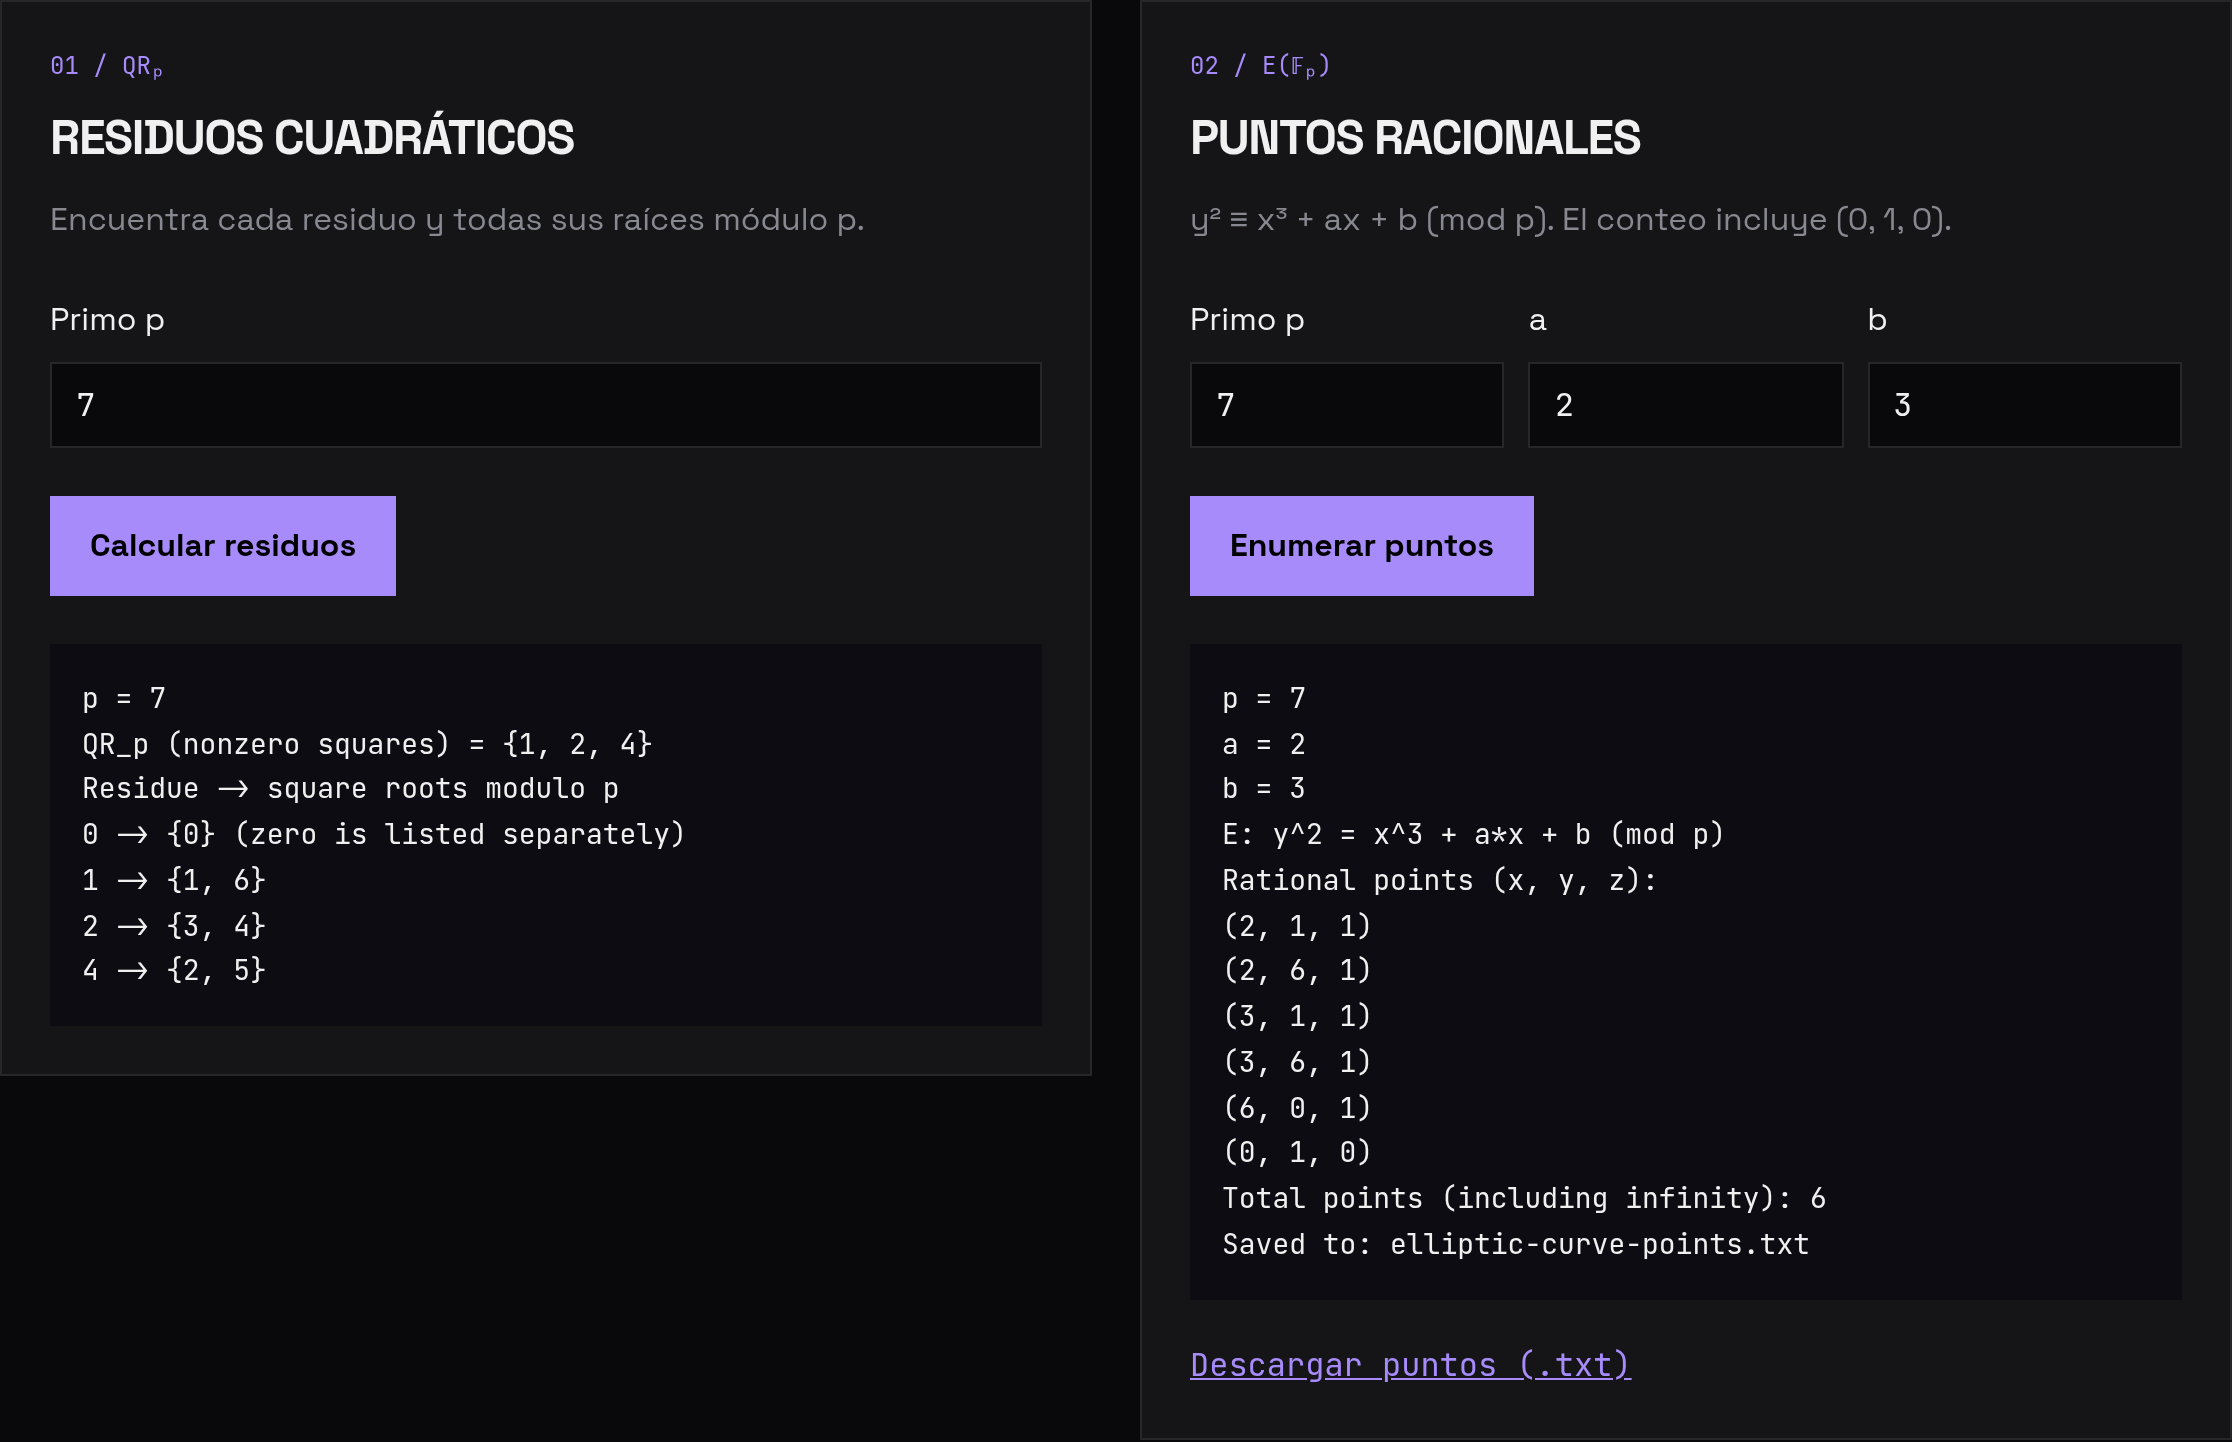
\includegraphics[width=\linewidth,height=0.88\textheight,keepaspectratio]{assets/capturas/final-web-puntos.png}
\end{center}
\clearpage
\section*{Captura de la web: operaciones}
\begin{center}
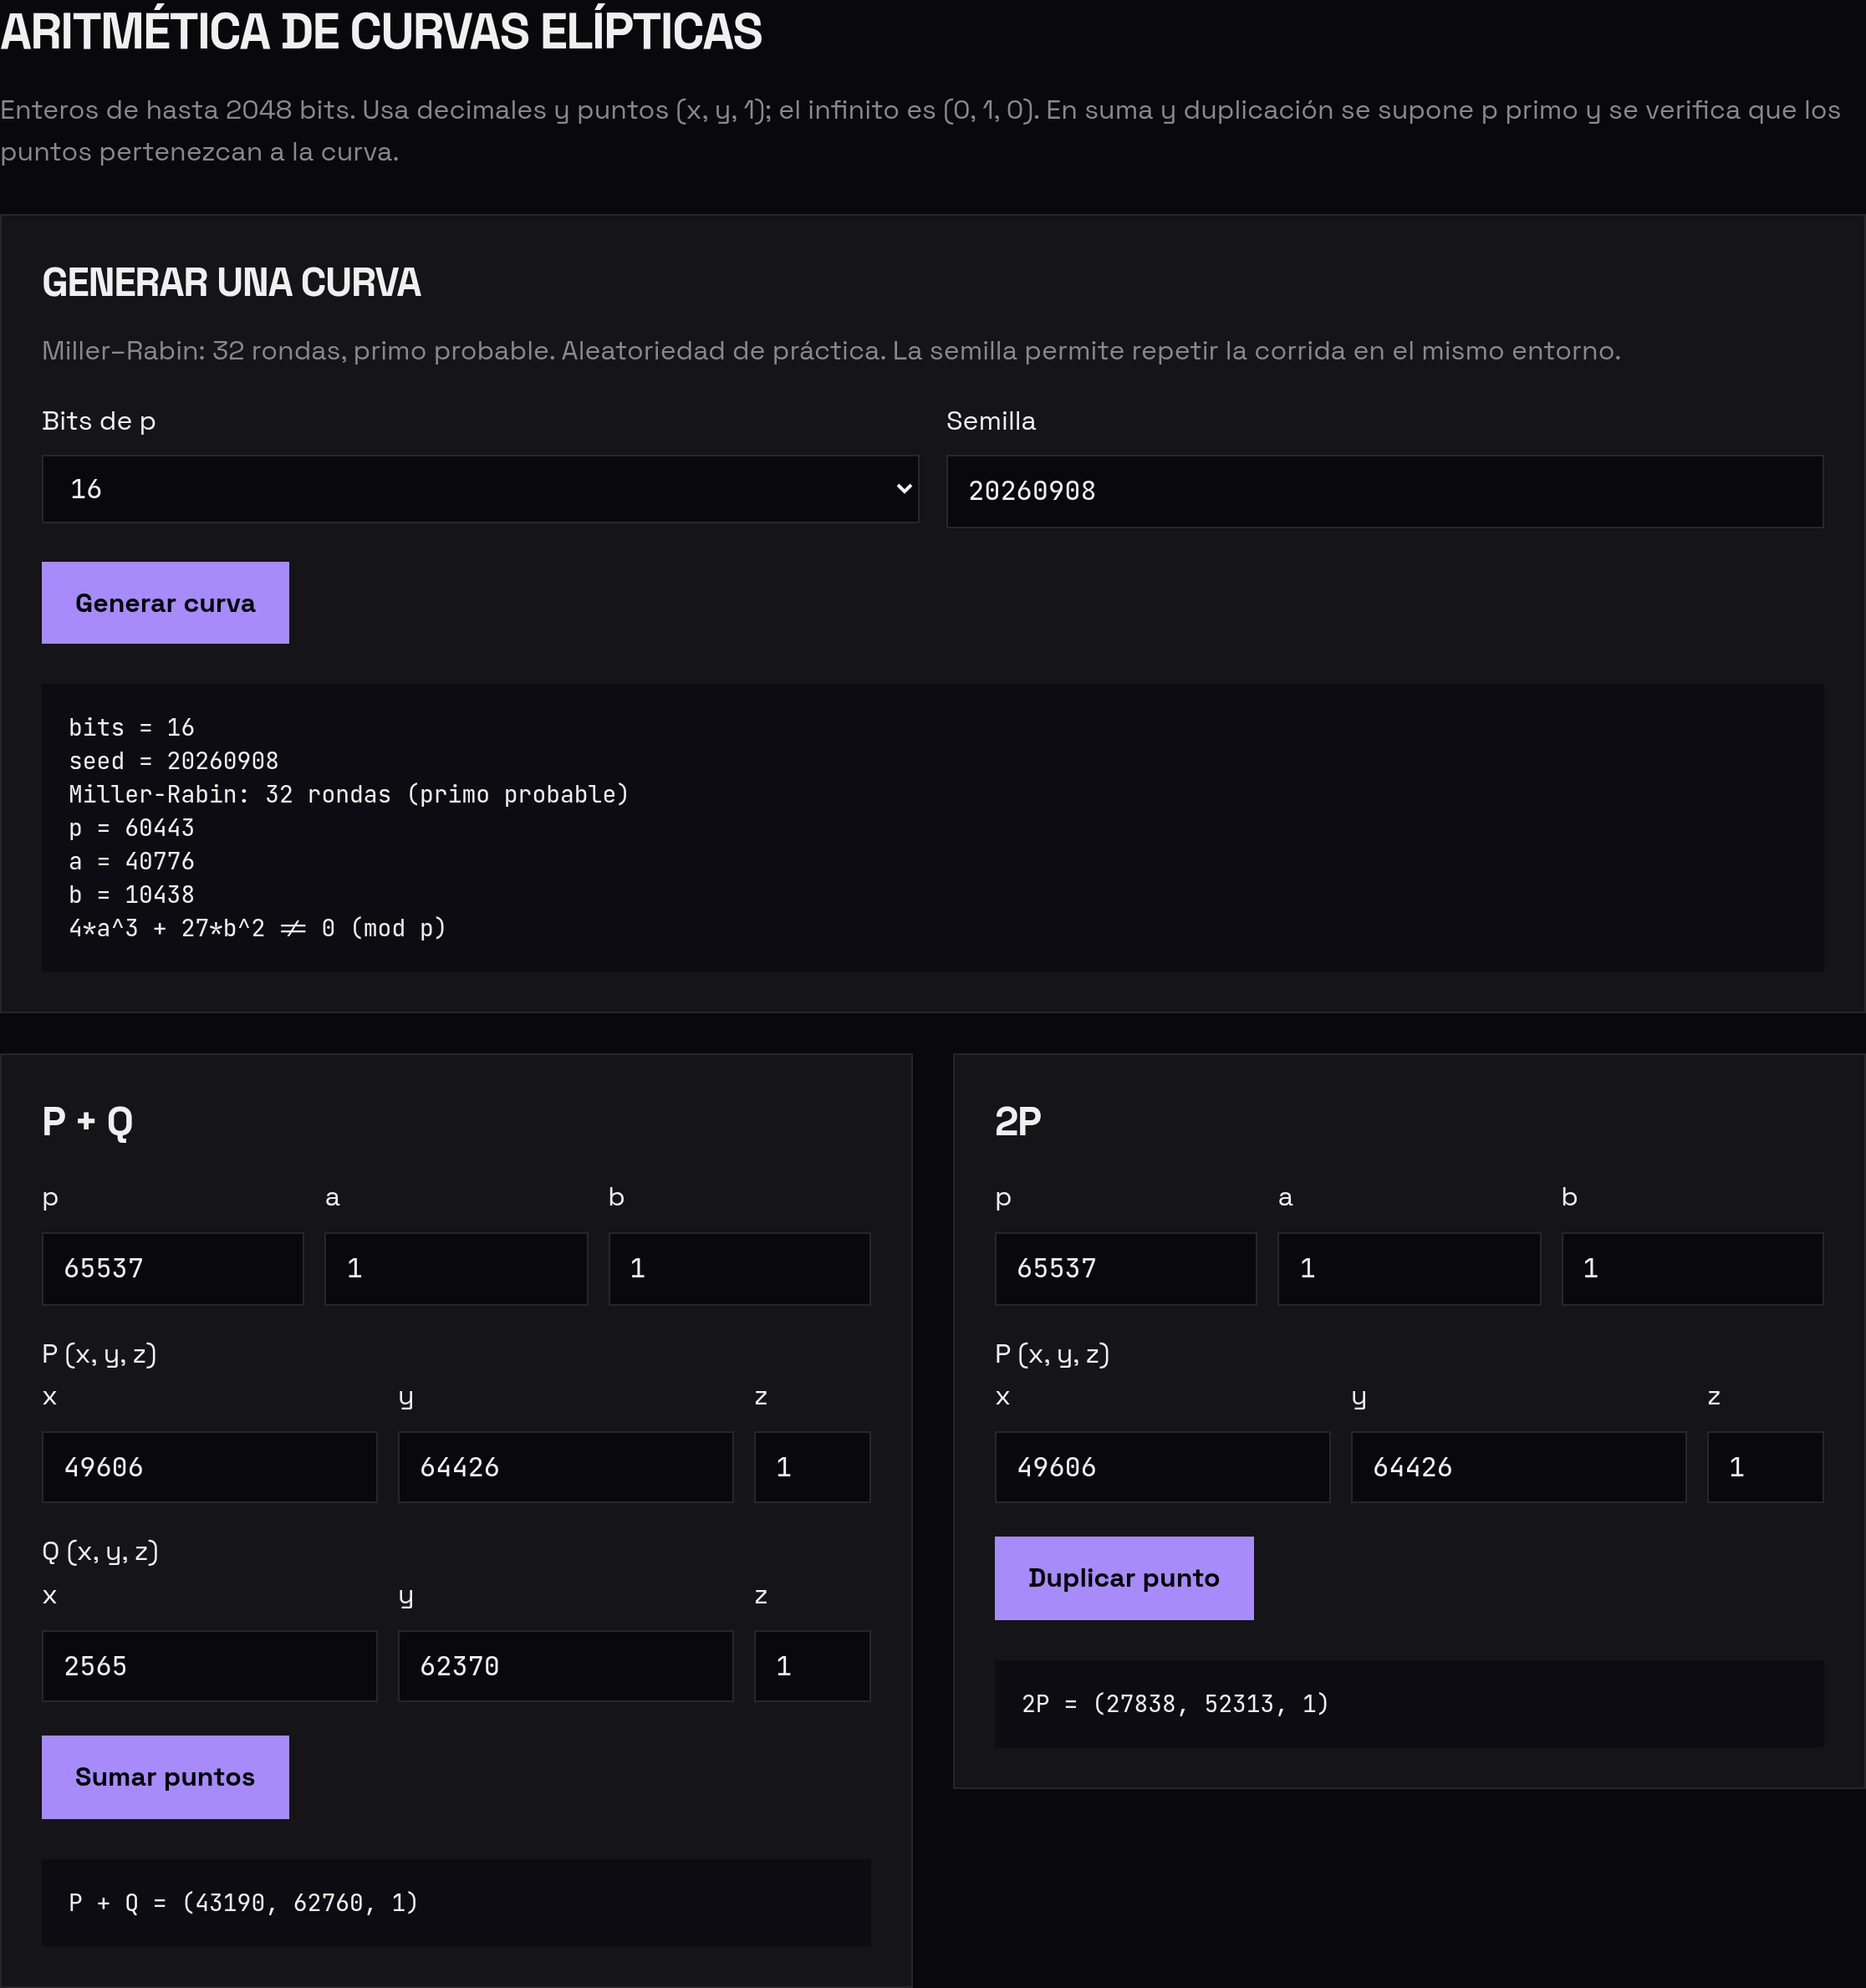
\includegraphics[width=\linewidth,height=0.88\textheight,keepaspectratio]{assets/capturas/final-web-aritmetica.png}
\end{center}
